\cleardoublepage

\lgf{\chapter{LA REPRESENTATION DE LA DONNEE}}
\lge{\chapter{THE REPRESENTATION OF DATA}}

\section{Introduction}
     \vspace{1em}

\lgf{Envoyer une donnée sur un réseau n’est pas aussi simple que l’on croit.}
\lge{Sending data over a network is not as simple as it seems.}
     \vspace{1em}

 \begin{wrapfigure}{r}{3cm}
\Youtube{https://youtu.be/k-RhgiwKx2M}
\end{wrapfigure}

\lgf{Il faut faire la différence entre le format utilisé pour stocker des données dans la mémoire de l'ordinateur et celui employé pour l'envoyer à une autre machine. En effet, chaque machine à sa propre représentation souvent liée aux capacités de leur processeur. Cela est surtout vrai pour les nombres. Ils peuvent être stockés sur un nombre de bits plus ou moins important ou peuvent être représentés en mémoire de manière optimisée pour accélérer leur traitement. }
\lge{There is a difference between the format used to store data in the computer's memory and the one used to send it to another machine. Indeed, each machine has its own representation often linked to the capacities of their processor. This is especially true for numbers. They can be stored on a more or less important number of bits or can be represented in memory in an optimized way to accelerate their treatment. }


\lgf{En revanche, la représentation des chaînes de caractères (non accentués) est relativement uniforme car elle se base sur le code ASCII qui est le même pour tous les ordinateurs. Un texte de base est facilement compréhensible par toutes les machines. Une solution serait donc de n'utiliser que des chaînes de caractères. }
\lge{On the other hand, the representation of (unaccented) character strings is relatively uniform because it is based on the ASCII code which is the same for all computers. A basic text is easily understandable by all machines. A solution would therefore be to use only strings of characters. }

     \vspace{1em}

\lgf{Par exemple, si l’on veut envoyer l'entier ayant pour valeur 123, il existe plusieurs représentations possibles :}
\lge{For example, if we want to send the integer with the value 123, there are several possible representations:}

\begin{itemize}
\item 
    \lgf{envoyer une chaîne de caractères ”123” contenant les chiffres du nombre ;}
    \lge{send a string "123" containing the digits of the number;}
\item 
    \lgf{envoyer la valeur binaire 1111011.}
    \lge{send the binary value 1111011.}
\end{itemize}

     \vspace{1em}

\lgf{On voit que juste pour transmettre une simple valeur stockée dans la mémoire d'un ordinateur, il existe plusieurs options et évidemment pour que cette valeur soit interprétée de la bonne façon, il faut que les deux extrémités se soient mises d'accord sur une représentation.}
\lge{We see that just to transmit a simple value stored in the memory of a computer, there are several options and obviously for this value to be interpreted in the right way, it is necessary that both ends have agreed on a representation.}

\lgf{Quand on veut transmettre plusieurs valeurs, c'est-à-dire quand on a des données structurées, d'autres problèmes surviennent.}
\lge{When you want to transmit several values, i.e. when you have structured data, other problems arise.}

\lgf{Par exemple : quelle est la taille des blocs que l’on va transmettre ? Comment indiquer la fin de la transmission ? Pour une chaîne de caractères, comment indiquer qu’elle se termine ? Autre exemple : si l'on veut transmettre "12" puis "3", comment faire pour que l'autre extrémité ne comprenne pas "123" ?}
\lge{For example: what is the size of the blocks we are going to transmit? How to indicate the end of the transmission? For a string, how to indicate that it ends ? Another example : if we want to transmit "12" and then "3", how do we make sure that the other end does not include "123"?}

     \vspace{1em}


\lgf{Pour que la transmission se fasse correctement, il faut que l’émetteur et le récepteur adoptent les mêmes conventions. Quand il s’agit d’un ensemble de données, il faut être capable de les séparer. Avec les tableurs, une première méthode est possible avec la notation \ac{CSV} Comme son nom l’indique, les valeurs sont séparées par des virgules. Les valeurs sont représentées par des chaînes de caractères. Les textes sont différenciés des valeurs numériques, par l’utilisation de guillemets. Ainsi, 123 sera interprété comme un nombre et ”123” comme un texte.}
\lge{In order for the transmission to take place correctly, the sender and receiver must adopt the same conventions. When it is a question of a set of data, it is necessary to be able to separate them. With spreadsheets, a first method is possible with the notation \ac{CSV} As its name indicates, the values are separated by commas. The values are represented by strings. The texts are differentiated from the numerical values by the use of quotation marks. Thus, 123 will be interpreted as a number and "123" as a text.}

\lgf{Si cette représentation est adaptée aux tableurs, elle est relativement pauvre car elle ne permet de représenter que des valeurs sur des lignes et des colonnes. Pour les usages du Web, il a fallu trouver un format plus souple permettant de représenter des structures de données complexes. Évidemment, comme rien n'est simple, il en existe plusieurs et les applications échangeant des données devront utiliser le même.}
\lge{If this representation is adapted to spreadsheets, it is relatively poor because it only allows to represent values on rows and columns. For Web uses, it was necessary to find a more flexible format allowing to represent complex data structures. Obviously, as nothing is simple, there are several of them and applications exchanging data will have to use the same one.}


     \vspace{1em}


\lgf{On voit que l'envoi de la chaîne de caractères ne suffit pas, il faut la formater pour que le récepteur puisse trouver le type de la donnée transmise, qu'un nombre ne soit pas interprété comme une chaîne de caractères, qu'une chaîne de caractères reste une chaîne de caractères même si elle ne contient que des chiffres.  }
\lge{We can see that sending the string is not enough, it must be formatted so that the receiver can find the type of the transmitted data, so that a number is not interpreted as a string, so that a string remains a string even if it contains only numbers.  }

    \vspace{1em}
   
\lgf{\section{La \Index{sérialisation}}}
\lge{\section{The \Index{serialization}}}

\lgf{Sous ce nom barbare se cache la méthode utilisée pour transmettre 
des données d’un ordinateur à un autre. Une donnée peut être simple (un nombre, un texte) ou plus complexe (un tableau, une structure...).  Elle est stockée dans la mémoire de l'ordinateur suivant une représentation qui lui est propre. Par exemple, la taille des entiers peut varier d'une technologie de processeur à une autre, l'ordre des octets dans un nombre peut aussi être différente (little et big endian).  Pour des structures complexes comme les tableaux, les éléments peuvent être rangés à différents emplacements de la mémoire. }
\lge{Under this barbaric name hides the method used to transmit 
data from one computer to another. A data can be simple (a number, a text) or more complex (an array, a structure...). It is stored in the computer's memory according to a representation that is specific to it. For example, the size of integers can vary from one processor technology to another, the order of bytes in a number can also be different (little and big endian).  For complex structures such as arrays, the elements can be stored in different locations in the memory. }


\lgf{La sérialisation consiste à transformer une structure de données en une séquence qui pourra être transmise sur le réseau, stockée dans un fichier ou une base de données. L'opération inverse, consistant à reconstruire localement une structure de données, s'appelle désérialisation.}
\lge{Serialization consists of transforming a data structure into a sequence that can be transmitted over the network, stored in a file or a database. The opposite operation, consisting in locally reconstructing a data structure, is called deserialization.}

\lgf{Il existe plusieurs formats pour sérialiser les données. Ils peuvent être binaires mais ceux généralement utilisés sont basés sur des chaînes de caractères. En effet, la représentation \ac{ASCII} définissant les caractères de base et codée sur 7 bits est commune à l'ensemble des ordinateurs. L'autre avantage du code ASCII est qu'il est facilement lisible et simplifie la mise au point des programmes.  }
\lge{There are several formats for serializing data. They can be binary but those generally used are based on character strings. Indeed, the representation \ac{ASCII} defining the basic characters and coded on 7 bits is common to all the computers. The other advantage of the ASCII code is that it is easily readable and simplifies the development of programs.  }

\lgf{Wikipédia donne ce tableau (cf. figure~\vref{fig-ASCII}) des codes \ac{ASCII} datant de 1972 (une éternité en informatique) et recolorisé par nos soins.}
\lge{Wikipedia gives this table (cf. figure~ref{fig-ASCII}) of the codes dating from 1972 (an eternity in computing) and recolored by us.}


\begin{figure}[tbp]
\centerline{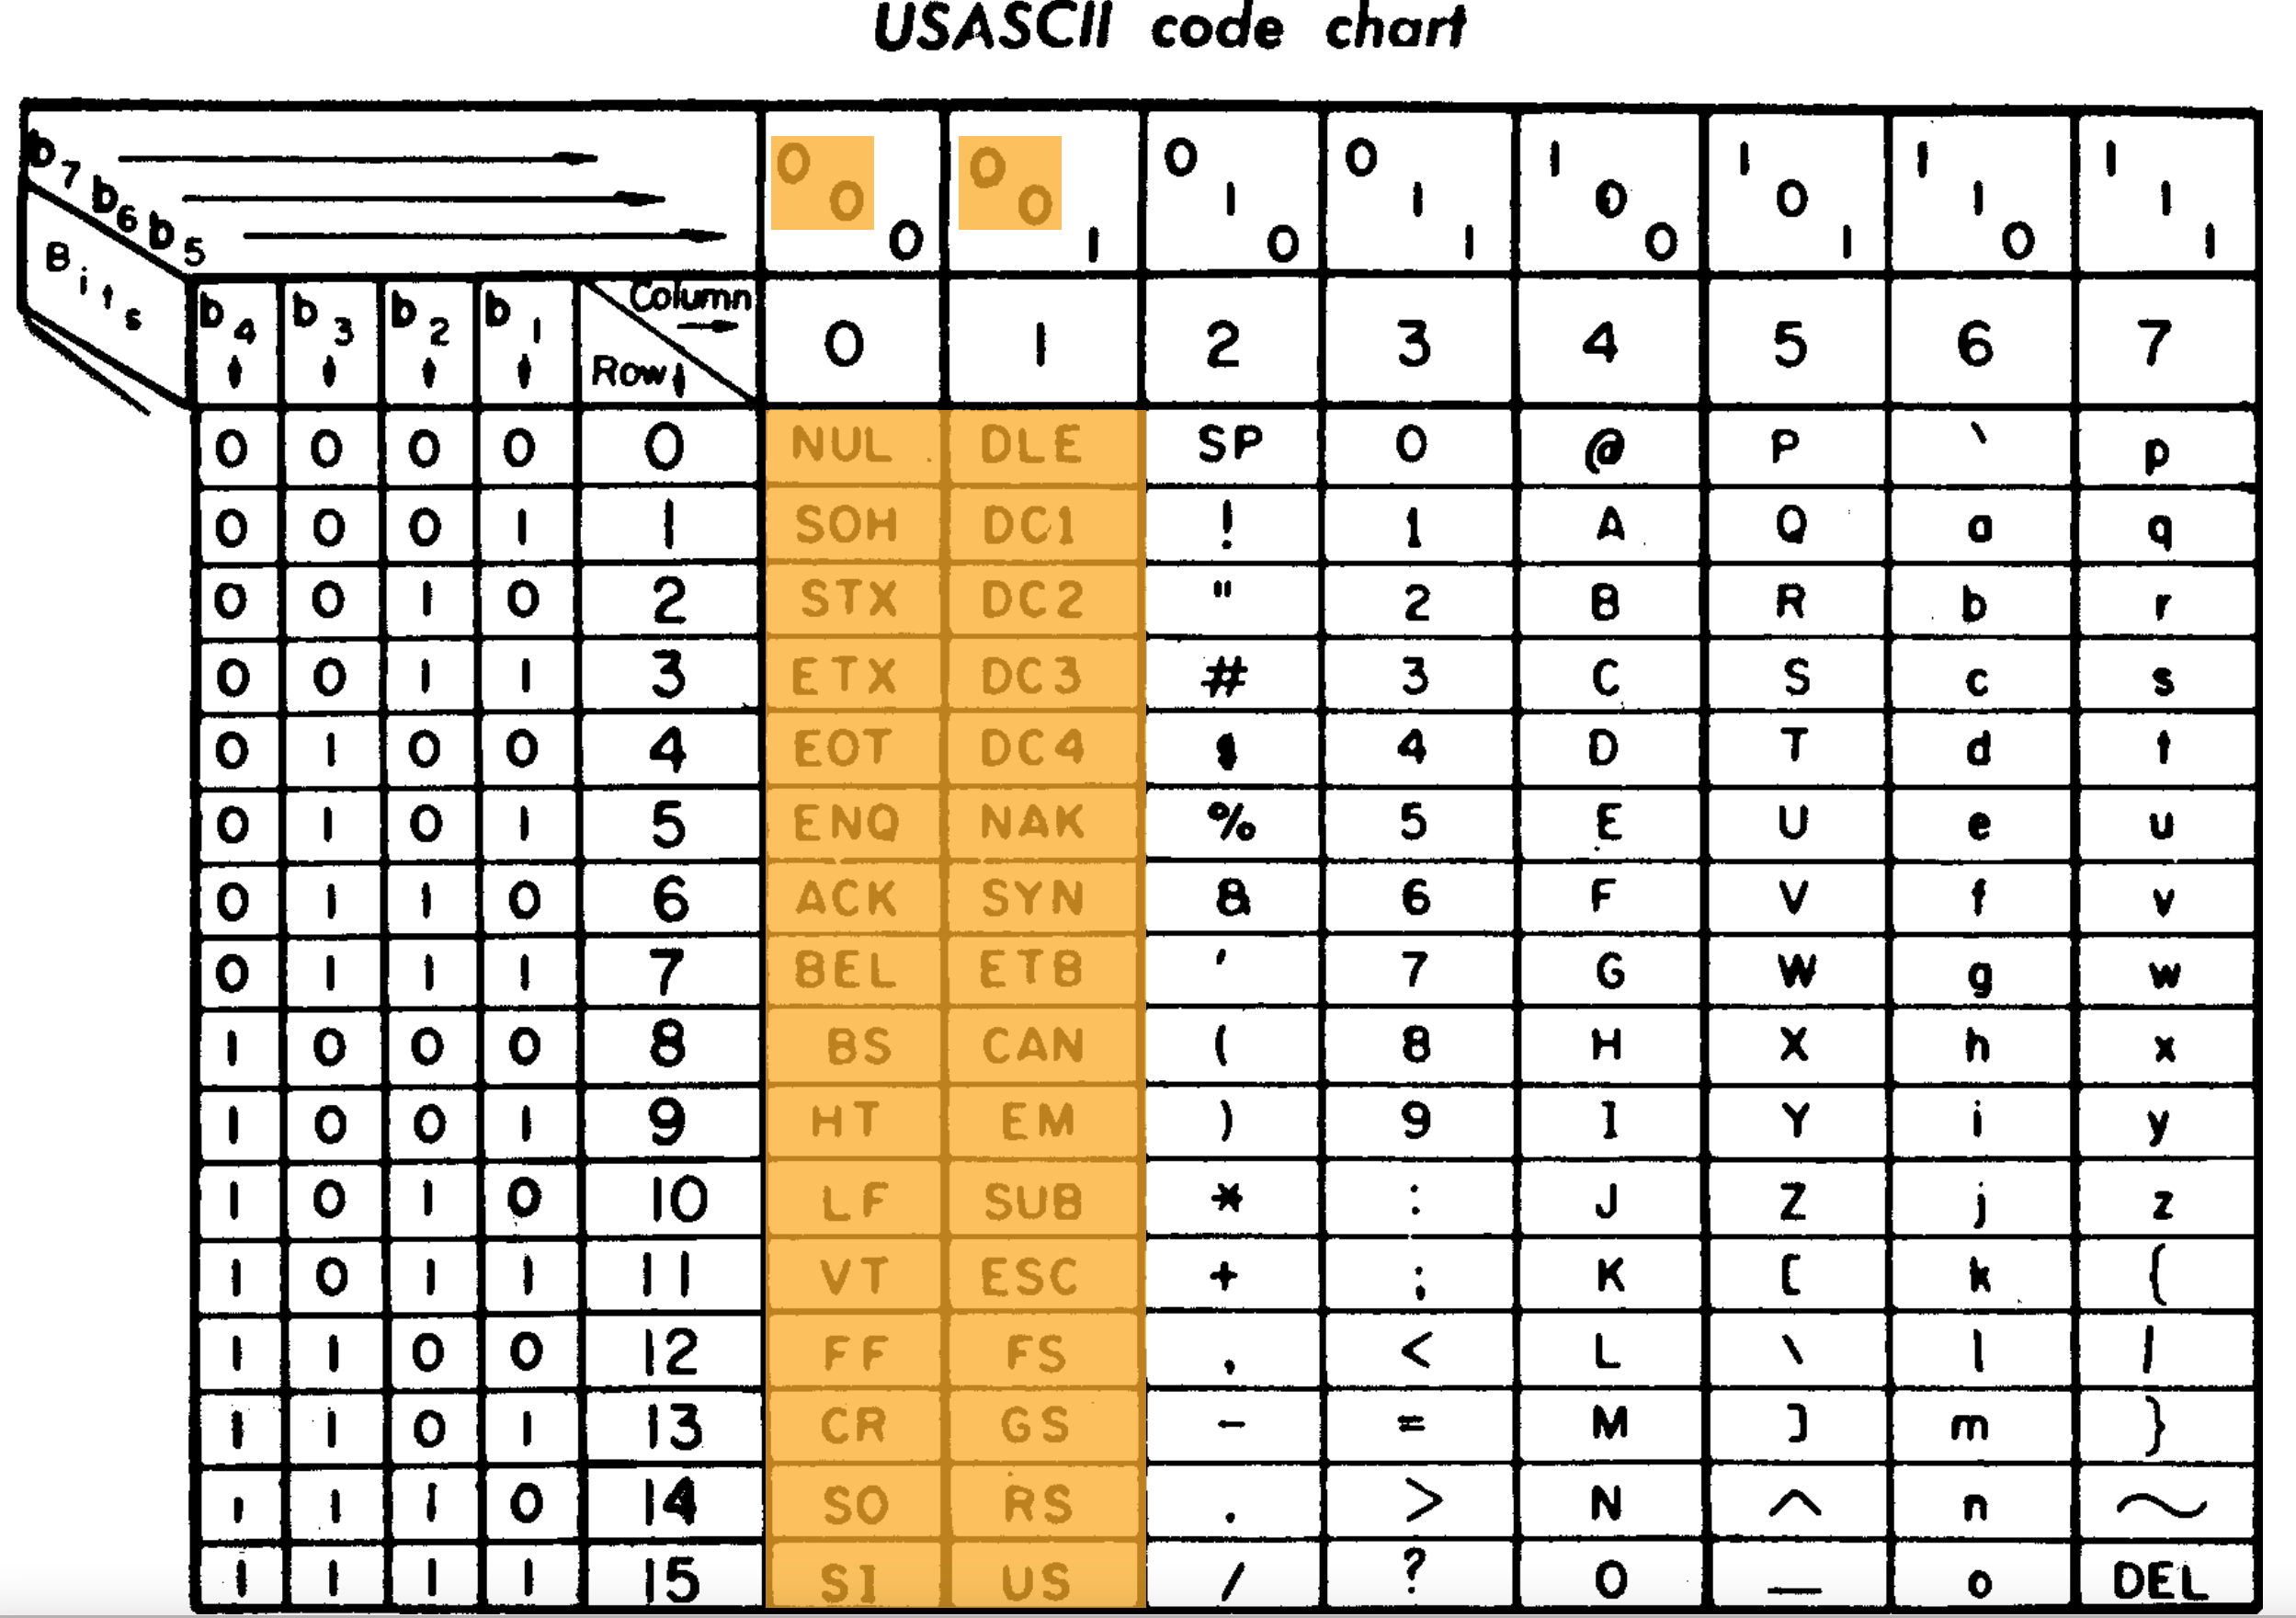
\includegraphics[width=1\columnwidth]{Pictures/Capture20.png}}
\lgf{\caption{Codage ASCII des caractères}}
\lge{\caption{ASCII character encoding}}
\label{fig-ASCII}
\end{figure}

\lgf{Les caractères en orange ne sont pas imprimables. Ils permettent de contrôler la communication des données ou de gérer l'affichage en revenant à la ligne. On les reconnait car la séquence binaire commence par 00X XXXX. On rappelle que le code ASCII est sur 7 bits ; le bit supplémentaire (bit de parité) conduisant à 1 octet était utilisé pour détecter des erreurs de transmission. Les valeurs de 0x30 à 0x39 codent les chiffres de 0 à 9. }
\lge{The characters in orange are not printable. They are used to control data communication or to manage the display by returning to the line. They can be recognized because the binary sequence starts with 00X XXXX. One recalls that the ASCII code is on 7 bits; the additional bit (parity bit) leading to 1 byte was used to detect transmission errors. The values from 0x30 to 0x39 code the digits from 0 to 9. }

\subsection*{Hexlify}

\lgf{En Python, il existe le module \Index{binascii} très pratique qui permet de convertir une séquence binaire en une chaîne de caractères ou inversement :}
\lge{In Python, there is the module \Index{binascii} very practical which makes it possible to convert a binary sequence into a character string or conversely:}
\begin{itemize}
\item 
    \lgf{\pfunction{binascii}{hexlify} prend un tableau d'octets et le convertit en une chaîne de caractères hexadécimaux plus lisible pour les spécialistes. Cela permet de visualiser n'importe quelle séquence de données. }
    \lge{\pfunction{binascii}{hexlify} takes an array of bytes and converts it to a more specialist-readable hexadecimal string. This allows you to view any sequence of data. }
\item 
    \lgf{\pfunction{binascii}{unhexify} fait l'inverse. Il prend une chaîne de caractères et la convertit en un tableau d'octets. Cela peut vous faciliter la programmation car, dans votre code, il est plus facile de manipuler des chaînes de caractères.}
    \lge{\pfunction{binascii}{unhexify} does the opposite. It takes a string and converts it to an array of bytes. This can make programming easier for you because in your code it is easier to manipulate strings.}

\end{itemize}
\lgf{Dans la suite, nous l'utiliserons pour manipuler des identifiants. Par exemple, ce bout de code illustre l'utilisation de ces fonctions :}
\lge{In the following, we will use these functions to manipulate identifiers. For example, this piece of code illustrates the use of these functions:}

\begin{python}
mac = lora.mac()
print ('devEUI: ',  binascii.hexlify(mac))

# create an OTAA authentication parameters
app_eui = binascii.unhexlify('70 B3 D5 7E D0 03 3A E3'.replace(' ',''))

\end{python}

\lgf{Comme nous le verrons par la suite, a fonction \pfunction{network}{lora.mac()} retourne un tableau d'octets. La fonction \pfunction{binascii}{hexlify} ligne suivante le convertit en chaîne de caractères pour un affichage plus propre. }
\lge{As we will see later, the function \pfunction{network}{lora.mac()} returns an array of bytes. The function \pfunction{binascii}{hexlify} in the follwoing line converts it to a string for a cleaner display. }

\lgf{Inversement, nous devons affecter une séquence binaire à la variable \texttt{app\_eui}. Nous mettons cette séquence hexadécimale en chaîne de caractères. Les espaces offrent plus de lisibilité. Ils sont retirés par la méthode replace et le résultat est converti en binaire grâce à \pfunction{binascii}{unhexify}}
\lge{Conversely, we must assign a binary sequence to the variable \texttt{app\_eui}. We put this hexadecimal sequence into a string. Spaces offer more readability. They are removed by the replace method and the result is converted into binary thanks to \pfunction{binascii}{unhexify}}

\section{Base64}

\lgf{Le passage d'une séquence binaire à une chaîne de caractères ASCII en représentant les valeurs conduit à un doublement du volume. Chaque bloc de 4 bits va conduire à produire un octet correspondant au caractère d'un chiffre ou d'une lettre de A à F. Le reste des codes n'est pas utilisé.}
\lge{The passage from a binary sequence to an ASCII character string representing the values leads to a doubling of the size. Each block of 4 bits will lead to produce a byte corresponding to the character of a digit or a letter from A to F. The rest of the codes are not used.}

\lgf{Le codage \Index{base64} offre un meilleur rendement en utilisant 64 bits pour coder les valeurs. Un dictionnaire fait la correspondance entre 64 valeurs et un caractère ASCII. Cependant, si l'on veut coder 4 octets, soit 32 bits, il faudra 5 blocs de 6 bits, et il y aura deux bits restants. Le symbole = indique que 2 bits sont ajoutés à la fin du codage. Donc, dans notre cas, il faudra ajouter deux symboles = comme le montre la figure ci-dessous :}
\lge{The encoding \Index{base64} offers a better performance by using 64 bits to encode the values. A dictionary maps 64 values to an ASCII character. However, if we want to encode 4 bytes, or 32 bits, we will need 5 blocks of 6 bits, and there will be 2 bits left. The symbol = indicates that 2 bits are added at the end of the coding. So, in our case, it will be necessary to add two symbols = as shown in the figure below:}

\begin{figure}[tbp]
\centerline{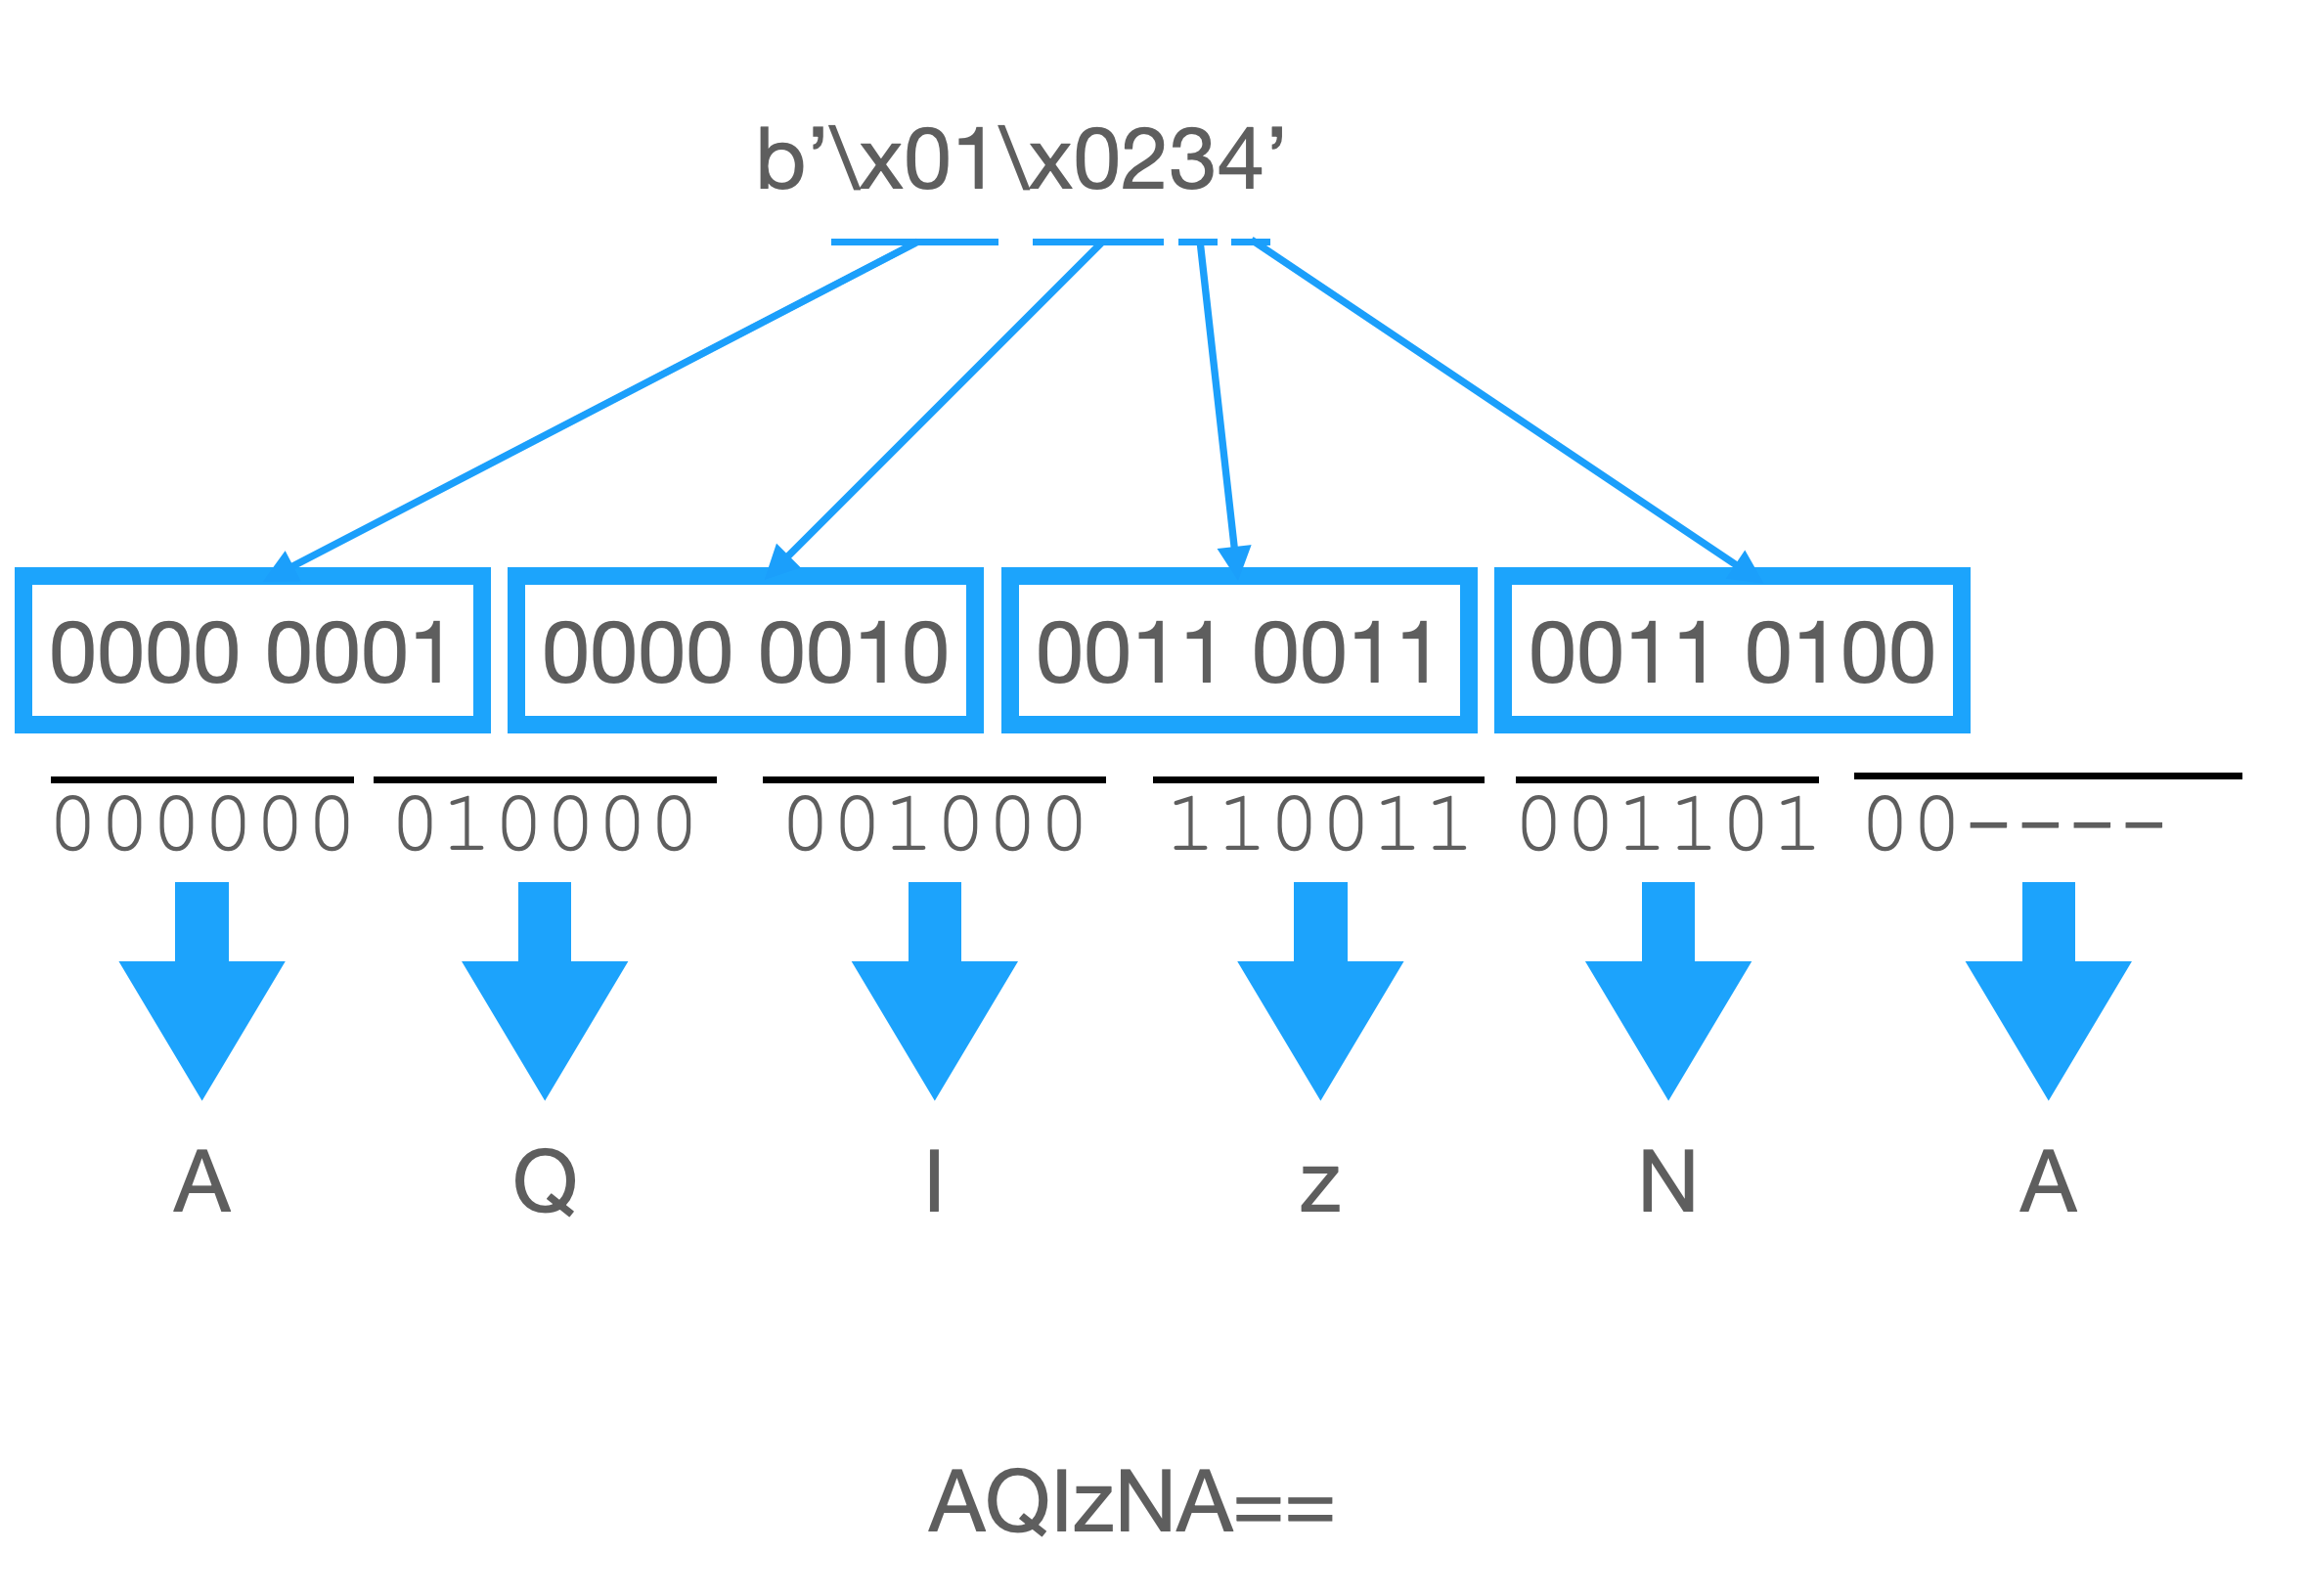
\includegraphics[width=1\columnwidth]{Pictures/Capture21.png}}
\lgf{\caption{Codage Base64 de données binaires}}
\lge{\caption{Base64 coding of binary data}}
\label{fig-base64}
\end{figure}

\lgf{On notera que pour les petites séquences, ce codage n'est pas meilleur que la transformation de la séquence hexadécimale en chaîne de caractères. Ici, il faut 8 caractères pour coder 4 octets. }
\lge{Note that for small sequences, this coding is not better than the transformation of the hexadecimal sequence into a string. Here, 8 characters are needed to encode 4 bytes. }

\lgf{Il existe beaucoup d'outils en ligne pour faire les conversions entre ces différentes représentations, comme le site \url{www.asciitohex.com}.}
\lge{There are many online tools to make conversions between these different representations, such as the site \url{www.asciitohex.com}.}

\lgf{\subsection*{Module Python : base64}}
\lge{\subsection*{Python module: base64}}

\lgf{En Python3, le module base64 permet de faire ces conversions.  Ce module est un peu susceptible sur les types de données à utiliser.}
\lge{In Python3, the base64 module allows to do these conversions.  This module is a bit touchy about the data types to use.}

\begin{python}[numbers=left,numbersep=5pt]
import base64

val = b"\x01\x0234"
ser = base64.b64encode(val)
print (ser)
print (ser.decode())
ori = base64.b64decode(ser)
print (ori)
\end{python}

\lgf{qui donne à l’exécution :}
\lge{which gives as a result of the execution :}

\begin{termc}[backgroundcolor=\color{backcolour}]
b'AQIzNA=='
AQIzNA==
b'\x01\x0234'
\end{termc}

\lgf{À noter que l'utilisation du \texttt{ser.\pfunction{str}{decode}()}, ligne 6, pour transformer une chaîne d'octets en chaîne de caractères, c'est-à-dire supprimer le \texttt{b} du début, peut être utilisé dans certains cas.}
\lge{Note that the use of \texttt{ser.\pfunction{str}{decode}()}, line 6, to transform a string of bytes into a string of characters, i.e. remove the \texttt{b} at the beginning, can be used in certain cases.}



\section{HTML}

\lgf{La sérialisation en chaînes de caractères (par exemple en Python via la commande \pfunction{binascii}{hexlify}) ou en Base64 concerne surtout des données binaires. Mais la donnée peut être aussi structurée, par exemple la page d'un tableur. Il faut donc formater le document pour éviter une fusion des différents champs.}
\lge{Serialization in strings (for example in Python via the command \pfunction{binascii}{hexlify}) or in Base64 concerns mainly binary data. But the data can also be structured, for example the page of a spreadsheet. The document must therefore be formatted to avoid merging the various fields.}


\lgf{\ac{HTML}, sans entrer dans les détails, définit un format où les champs sont repérés par un balisage.  Une balise de début est un mot clé entre \texttt{<>} et, pour une \Index{balise} de fin, le mot clé est précédé du caractère \texttt{/}. Par exemple, la figure~\vref{fig-HTML} avec le balisage, le premier paragraphe est formaté de cette manière dans le MOOC :}
\lge{\ac{HTML}, without going into detail,  defines a format where fields are marked up with markup.  A beginning tag is a keyword between \texttt{<>} and, for an ending \Index{tag}, the keyword is preceded by the character \texttt{/}. For example, the figure~\vref{fig-HTML} with the markup, the first paragraph is formatted this way in the MOOC:}


\begin{figure}[tbp]
\centerline{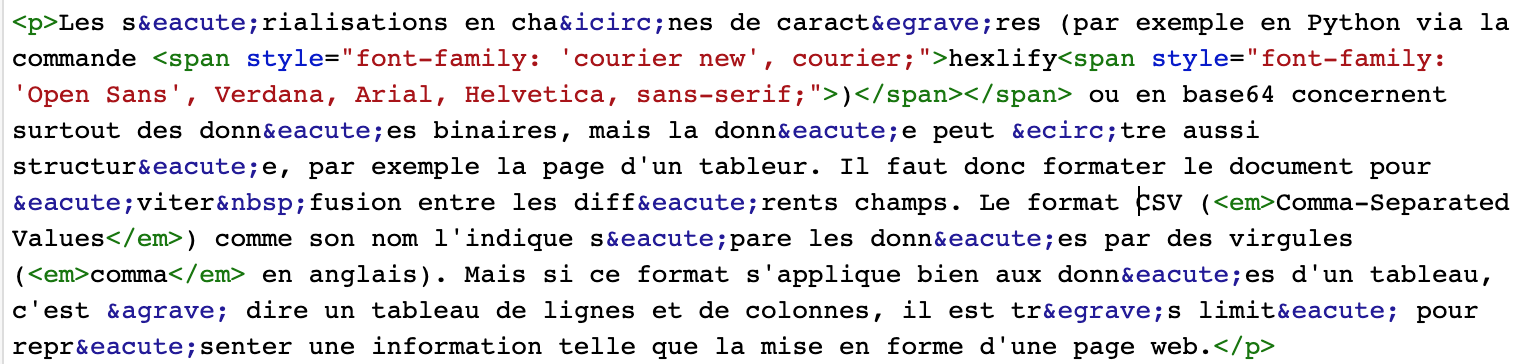
\includegraphics[width=1\columnwidth]{Pictures/Capture22.png}}
\lgf{\caption{Codage HTML d'une page Web}}
\lge{\caption{HTML coding of a Web page}}
\label{fig-HTML}
\end{figure}

\lgf{Les balises peuvent aussi prendre des arguments, comme la balise \Index{span} dans l'exemple précédent. Ainsi, si l'on regarde une page Web, comme indiqué figure~\vref{fig-Web-HTML}, le navigateur est capable de l'analyser pour trouver les \ac{URI} qu'elle contient. La balise \texttt{\Index{img}} indiquant qu'il s'agit d'une image, le client peut interroger le serveur pour l'afficher à l'écran. Ce format structuré de sérialisation nous permet de mettre en place une caractéristique de \ac{REST}, c'est-à-dire les liens entre ressources.}
\lge{Tags can also take arguments, like the \Index{span} tag in the previous example. Thus, if we look at a Web page, as shown in figure~\vref{fig-Web-HTML}, the browser is able to analyze it to find the \ac{URI} it contains. With the text tag indicating that it is an image, the client can query the server to display it on the screen. This structured serialization format allows us to implement a feature of \ac{REST}, i.e. the links between resources.}

\begin{figure}[tbp]
\centerline{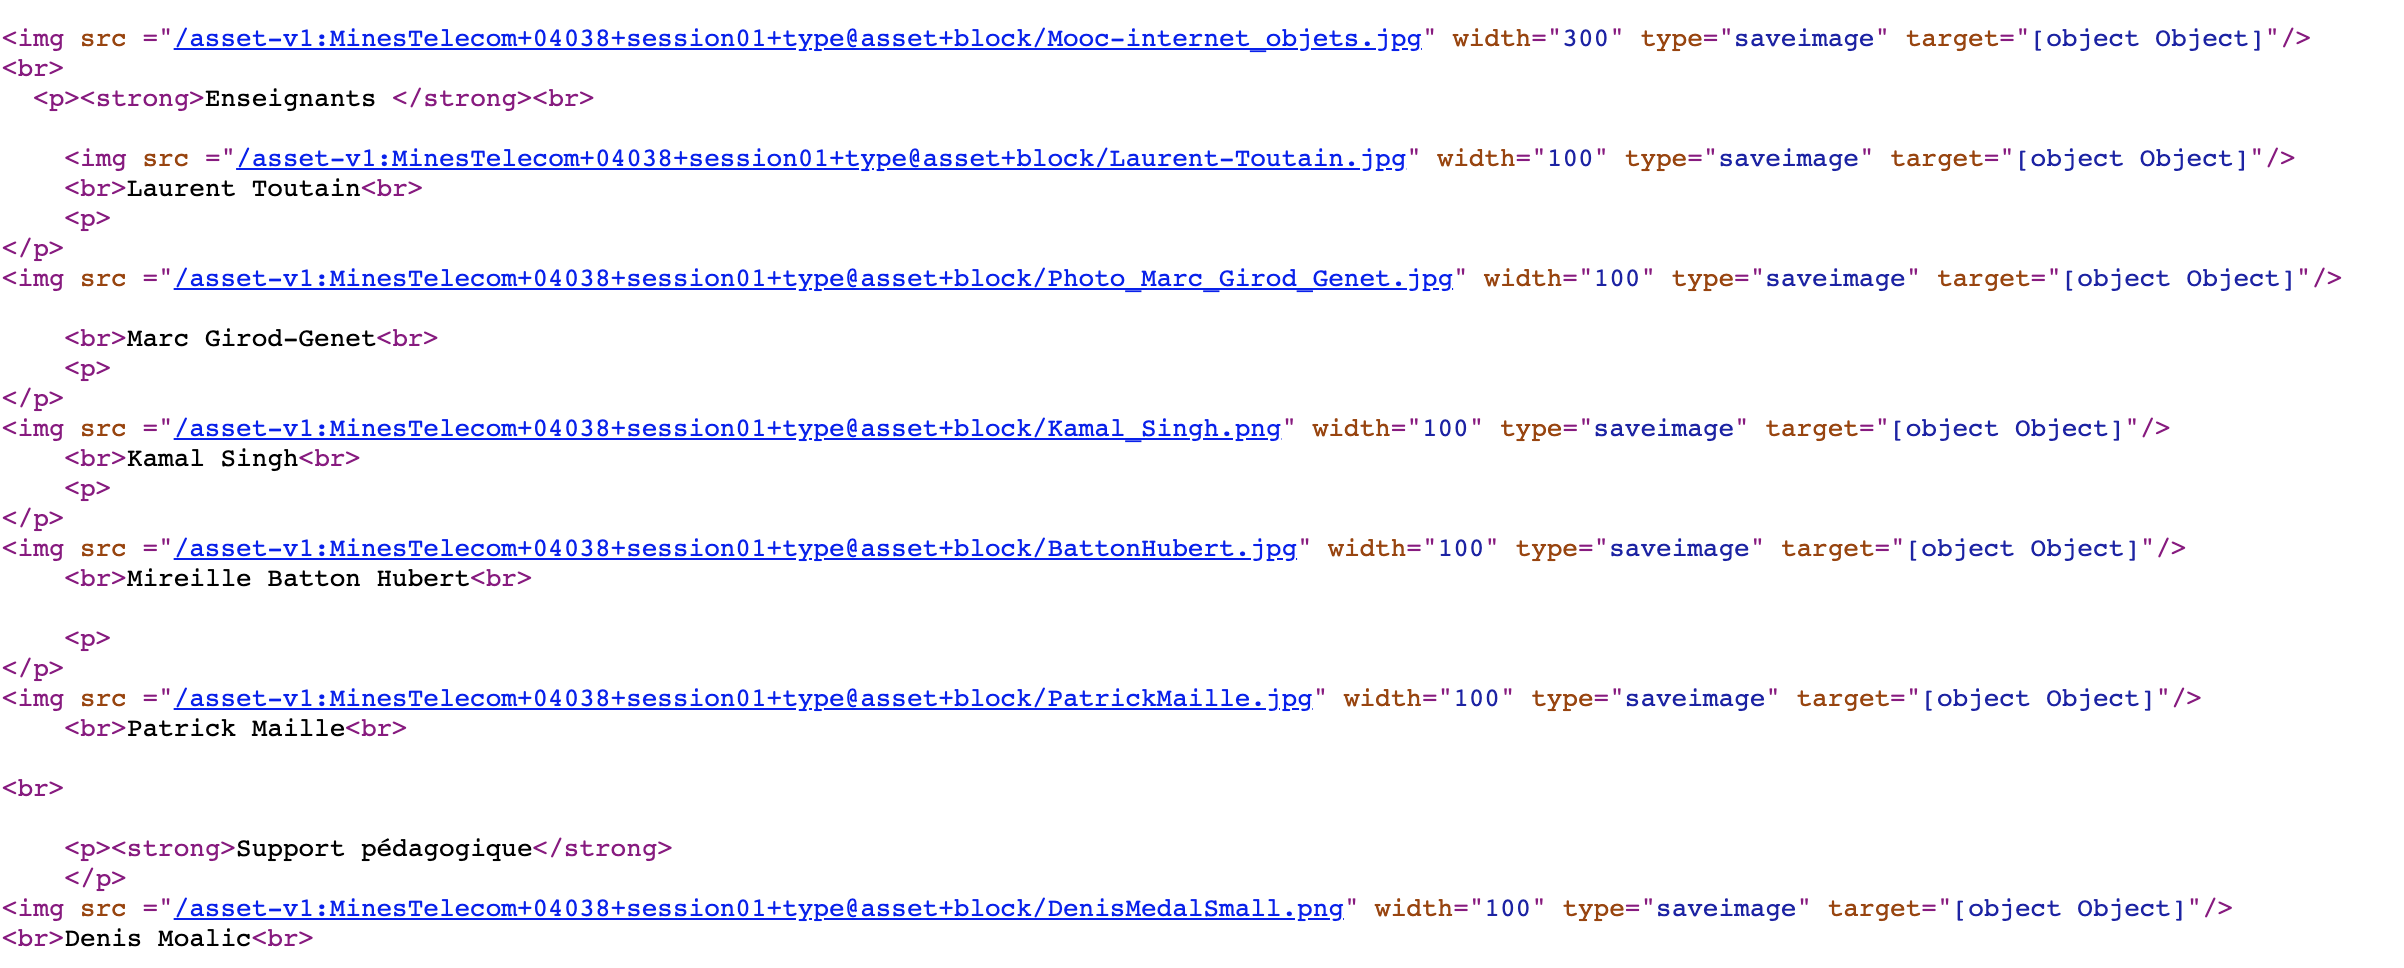
\includegraphics[width=1\columnwidth]{Pictures/Capture23.png}}
\lgf{\caption{Capture d'une page Web}}
\lge{\caption{Capture a web page}}
\label{fig-Web-HTML}
\end{figure}


\section{XML}

\lgf{Si \ac{HTML} est dédié au formatage à l'écran de données textuelles et à la navigation sur le Web. \ac{XML}\footnote{\url{https://www.w3.org/TR/xml/}} défini par le \ac{W3C}, est un format d’échange entre deux applications. Par exemple, pour échanger les notes des étudiants entre la plate-forme FUN et une autorité de certification des cours, on pourrait utiliser le format suivant~:}
\lge{If \ac{HTML} is dedicated to the formatting on screen of textual data and to the navigation on the Web. \ac{XML}\footnote{\url{https://www.w3.org/TR/xml/}} defined by the \ac{W3C}, is a format for exchange between two applications. For example, to exchange student grades between the FUN platform and a course certification authority, one could use the following format~:}

\begin{termc}[backgroundcolor=\color{palerod}]
<etudiant>
   <prenom>John</prenom>
   <nom>Deuf</nom>
   <note>18</note>
</etudiant>

\end{termc}

\lgf{Il est facile en lisant l'exemple de trouver le prénom, le nom et la note de l'étudiant. On peut noter qu'il n'y a pas de différence entre la note et le nom de l'élève. Il s'agit de caractères.}
\lge{It is easy by reading the example to find the student's first name, last name and grade. It can be noted that there is no difference between the grade and the student's name. They are characters.}

     \vspace{1em}

\lgf{S'il est syntaxiquement correct, rien ne dit que le créateur fournit quelque chose de correct qui pourra être interprété par une autre instance.  \ac{XML} peut inclure une grammaire ou un schéma qui est utilisé pour valider que les informations représentées dans le fichier sont non seulement syntaxiquement conformes au langage \ac{XML}, mais aussi conformes au schéma. Ce schéma va décrire les champs attendus et leur type (texte, nombre...). Vous pouvez accéder à ce cours si vous voulez en savoir plus sur les schémas \ac{XML}.}
\lge{If it is syntactically correct, there is no guarantee that the creator is providing something correct that can be interpreted by another instance.  \XML can include a grammar or schema that is used to validate that the information represented in the file is not only syntactically compliant with the language, but also complies with the schema. This schema will describe the expected fields and their type (text, number...). You can access this course if you want to know more about schemas.}

\lgf{Du point de vue de l’internet des objets, même si le XML pourrait être un bon candidat pour l’échange d’informations, il est un format trop lourd et donc énergivore. On peut noter que pour envoyer une note sur 20 qui, dans l'absolu, prendrait 6 bits, on transmet \texttt{<note>18</note>}, soit 15 caractères soit 120 bits! }
\lge{From the point of view of the Internet of Things, even if XML could be a good candidate for the exchange of information, it is too heavy a format and therefore energy consuming. We can note that to send a note out of 20 which, in the absolute, would take 6 bits, we transmit \texttt{<note>18</note>}, that is to say 15 characters or 120 bits! }

\section{JSON}

 \begin{wrapfigure}{r}{3cm}
\Youtube{https://youtu.be/IhZ9w6jWnq8}
\end{wrapfigure}

\lgf{\ac{JSON}  offre un moyen de structurer l’information de manière plus compacte que \ac{XML}. JSON s’impose comme le langage commun pour échanger les informations. A l’origine, JSON était utilisé par\Index{Javascriptt} pour échanger des informations ; par exemple, pour afficher en temps réel l’évolution des cours de la bourse ou pour afficher des graphiques dynamiques sur l’écran de l’utilisateur.}
\lge{\ac{JSON} offers a way to structure information in a more compact way than XML. JSON is emerging as the common language for exchanging information. Originally, JSON was used by \Index{Javascript} to exchange information; for example, to display in real time the evolution of stock exchange prices or to display dynamic graphs on the user's screen.}

\lgf{JSON \rfc{8259} est un format d’échange simple. Il définit 4 types de données :}
\lge{JSON \rfc{8259} is a simple exchange format. It defines 4 data types:}

\begin{itemize}
    \item 
        \lgf{nombre~: Les nombres sont composés de chiffres et peuvent être positifs, négatifs, entiers ou flottants.}
        \lge{Number: Numbers are composed of digits and can be positive, negative, integers or floats.}
    \item  
        \lgf{texte~: Le texte est délimité par des guillemets simples ou doubles.}
        \lge{Text: The text is delimited by single or double quotation marks.}
    \item  
        \lgf{\Index{tableau}~: Les tableaux sont des listes d’éléments séparés par des virgules et entourés de crochets.}
        \lge{\Index{Array}~: Arrays are lists of elements separated by commas and surrounded by square brackets.}
    \item  
        \lgf{\Index{objet}~: L’objet est une liste de paires composées d’une \Index{clé} et d’une valeur. La clé est une chaîne de caractères et la valeur peut être de n’importe quel type. La clé doit être unique à l’intérieur d’un objet, et référence entièrement la valeur qui la suit. Le couple clé - valeur est séparé par le caractère 2 points  \texttt{:}. Les éléments de l’objet sont séparés par des virgules. L'objet est délimité par des accolades.}
        \lge{\Index{Object}~: The object is a list of pairs composed of an \Index{key} and a value. The key is a string and the value can be of any type. The key must be unique within an object, and fully references the value that follows it. The couple key - value is separated by the colon character \texttt{:}. The elements of the object are separated by commas. The object is delimited by braces.}
\end{itemize}

\lgf{Par exemple, quelques structures \ac{JSON} :}
\lge{For example, some \ac{JSON} structures :}

\begin{itemize}
    \item 
        \lgf{\texttt{[1, -2, 0.3, 4e1]} est un tableau qui contient 4 nombres ;}
        \lge{\texttt{[1, -2, 0.3, 4e1]} is an array that contains 4 numbers;}
    \item  
        \lgf{\texttt{[1, ”2”, ”34”]} est un tableau contenant un nombre et deux chaines de caractères ;}
        \lge{\texttt{[1, "2", "34"]} is an array containing a number and two strings;}
    \item  
        \lgf{\texttt{[1, [2, 3 , ”4”]]} est un tableau de deux éléments dont le second est également un tableau de 3 éléments ;}
        \lge{\texttt{[1, [2, 3 , "4"]]} is an array of two elements whose second element is also an array of 3 elements;}
    \item  
        \lgf{\texttt{\{ ”couleur” : [34, 16, 3]\}} est un objet qui contient un élément et la valeur est un tableau ; }
        \lge{\texttt{\{ "color": [34, 16, 3]\}} is an object that contains an element and the value is an array; }
    \item  
        \lgf{\texttt{\{ ”name” : ”bob”, ”age” : 30\}} est un objet qui contient deux éléments référencés par les chaînes de caractères (ou index)  ”name” et ”age”.}
     
        \lgf{L’ordre dans lequel sont placés les éléments est indifférent. \texttt{\{”age” : 30, ”name” : ”bob”\}} est équivalent au dernier exemple. }
    
        \lgf{ Cela impose que l’index utilisé pour accéder à une valeur doit être unique dans la structure objet \texttt{\{”name” : ”bob”, ”name” : ”alice”}\} est interdit.}
        
        \lge{\texttt{ \{"name" : "bob", "age" : 30\}} is an object that contains two elements referenced by the strings (or index) "name" and "age".}
     
        \lge{The order in which the elements are placed is irrelevant. For example, \texttt{\{"age": 30, "name": "bob"\}} is equivalent to the last example. }
    
        \lge{This imposes that the index used to access a value must be unique in the object structure : \texttt{\{"name" : "bob", "name" : "alice"\}} is prohibited.}
\end{itemize}

     \vspace{1em}

\lgf{Le listing suivant donne un exemple de structure JSON tirée du \rfc{8259}. Il contient un objet JSON avec une seule clé \texttt{”Image”}. La valeur de cette clé est une autre structure qui contient six éléments. }
\lge{The following listing gives an example of a JSON structure from the \rfc{8259}. It contains a JSON object with a single key \texttt{"Image"}. The value of this key is another structure that contains six elements. }

\begin{termc}[backgroundcolor=\color{palerod}, language=json]
{
"Image": {
      "Width": 800,
      "Height": 600,
      "Title": "View from 15th Floor",
      "Thumbnail": {   
           "Url": "http://www.example.com/image/481989943",
           "Height": 125,
           "Width": 100
       },
       "Animated" : false,
       "IDs": [11, 943, 234, 38793]
    }
}
\end{termc}

\lgf{Le balisage par clé est un élément fondamental dans la structure des données. Il est primordial d'être cohérent et d'assurer une concordance entre émetteur et récepteur sur l'intitulé de la clé pour pouvoir récupérer l'information voulue. De la même façon, il faut s'accorder sur les unités de mesure : une interprétation d'une mesure en centimètre alors qu'elle est en pixel peut être désastreux ; c'est un problème d'interopérabilité.}
\lge{Key markup is a fundamental element in the structure of data. It is essential to be consistent and to ensure that the sender and receiver agree on the name of the key in order to be able to retrieve the desired information. In the same way, it is necessary to agree on the units of measurement: an interpretation of a measurement in centimeters when it is in pixels can be disastrous; it is an interoperability problem.}


     \vspace{1em}

\lgf{JSON est facilement exploitable dans d’autres langages. Par exemple en Python, le module JSON peut être utilisé pour convertir une structure JSON qui est une chaîne ASCII en une représentation interne Python. Les tableaux sont convertis en listes et les objets en dictionnaires.}
\lge{JSON is easily exploitable in other languages. For example in Python, the JSON module can be used to convert a JSON structure that is an ASCII string into a Python internal representation. Arrays are converted into lists and objects into dictionaries.}

     \vspace{1em}
     \pythonlst{example\_json.py}

\lgf{Le programme \pprog{example\_json.py}{cbor-example} reprend la structure précédente. La variable \texttt{struct\_python} est une structure Python. On peut voir que les valeurs pour \texttt{"Animated"} et \texttt{"Copyright"} sont les mots clé Python \texttt{False} (avec un F majuscule) et \texttt{None}. Le programme affiche deux fois cette valeur avec la commande standard \texttt{print} puis avec le module \pfunction{pprint}{pprint} pour avoir un affichage plus lisible. On peut remarquer que l'ordre d'affichage des clés est différent. Comme \texttt{"Title"} était défini deux fois, seul le dernier est conservé dans la structure Python.}
\lge{The program \pprog{example\_json.py}{cbor-example} uses the previous structure. The variable \texttt{struct\_python} is a Python structure. We can see that the values for \texttt{"Animated"} and \texttt{"Copyright"} are the Python keywords \texttt{False} (with a capital F) and \texttt{None}. The program displays this value twice with the standard command \texttt{print} then with the module \pfunction{pprint}{pprint} to have a more readable display. You can notice that the order of display of the keys is different. As \texttt{"Title"} was defined twice, only the last one is kept in the Python structure.}

\begin{termc}[backgroundcolor=\color{palerod}, language=json, basicstyle=\ttfamily\tiny]
{'Image': {'IDs': [17, 2371, 234, 38793], 'Height': 600, 'Animated': False, 'Title': 'Empty picture', 'Thumbnail': 
{'Url': 'http://www.example.com/image/481989943', 'Width': 100, 'Height': 125}, 'Width': 800, 'Copyright': None}}
{'Image': {'Animated': False,
           'Copyright': None,
           'Height': 600,
           'IDs': [17, 2371, 234, 38793],
           'Thumbnail': {'Height': 125,
                         'Url': 'http://www.example.com/image/481989943',
                         'Width': 100},
           'Title': 'Empty picture',
           'Width': 800}}
\end{termc}

\lgf{Grâce à la fonction \pfunction{json}{dumps} du module \texttt{json}, la variable \texttt{struct\_python} est transformée en JSON. Les mots clé  \texttt{False} et  \texttt{None} sont remplacés par  \texttt{false} et  \texttt{null}. Le programme affiche une chaîne de caractères.}
\lge{Thanks to the function \pfunction{json}{dumps} of the module \texttt{json}, the variable \texttt{struct\_python} is transformed into JSON. The keywords \texttt{False} and \texttt{None} are replaced by \texttt{false} and \texttt{null}. The program displays a string.}

\begin{termc}[backgroundcolor=\color{palerod}, language=json, basicstyle=\ttfamily\tiny]
{"Image": {"IDs": [17, 2371, 234, 38793], "Height": 600, "Animated": false, "Title": "Empty picture", "Thumbnail": 
{"Url": "http://www.example.com/image/481989943", "Width": 100, "Height": 125}, "Width": 800, "Copyright": null}}
\end{termc}

\lgf{Pour le retransformer, de JSON en variable Python, on utilise la fonction inverse \pfunction{json}{loads} qui traduit une chaîne de caractères en variable Python.}
\lge{To transform it back, from JSON to Python variable, we use the inverse function \pfunction{json}{loads} which translates a string into a Python variable.}

\begin{termc}[backgroundcolor=\color{palerod}, language=json, basicstyle=\ttfamily\tiny]
{'Image': {'Animated': False,
           'Copyright': None,
           'Height': 600,
           'IDs': [17, 2371, 234, 38793],
           'Thumbnail': {'Height': 125,
                         'Url': 'http://www.example.com/image/481989943',
                         'Width': 100},
           'Title': 'Empty picture',
           'Width': 800}}
\end{termc}


\lgf{Les autres langues de programmation possèdent également leur propre bibliothèque pour effectuer la traduction.}
\lge{Other programming languages also have their own libraries for translation.}

     \vspace{1em}

\lgf{Par rapport à \ac{XML}, \ac{JSON} est beaucoup plus permissif et manque de formalisme pour décrire la structure. \ac{JSON-LD} défini par le \ac{W3C} renforce l’interopérabilité de JSON en introduisant des clés spécifiques décrivant la structure des données, une référence aux unités, etc. Nous verrons ces concepts dans la suite du cours.}
\lge{Compared to \ac{XML}, \ac{JSON} is much more permissive and lacks a formalism to describe the structure. The \ac{JSON-LD} defined by the W3C reinforces the interoperability of JSON by introducing specific keys describing the data structure, a reference to units, etc. We will see these concepts in the rest of the course.}

\section{CBOR}

\begin{wrapfigure}{r}{3cm}
\Youtube{https://youtu.be/thSWuJ-1ld0}
\end{wrapfigure}

\lgf{\ac{JSON} et \ac{CBOR} sont tous les deux des modes de codage de la donnée.}
\lge{\ac{JSON} and \ac{CBOR} are both data encoding modes.}

\lgf{\ac{JSON} introduit une notation très flexible permettant de représenter toutes les structures de données. Le choix de l'\acs{ASCII} rend ce format universel et n'importe quel ordinateur pourra le comprendre. Mais l'utilisation de l'\acs{ASCII} ne permet pas de transmettre de manière optimale l'information sur un réseau. Quand les réseaux ont un débit raisonnable, cela ne pose pas de problème. Quand on en vient à l'internet des objets, il faut prendre en compte la capacité de traitement limité des équipements et la faible taille des messages échangés.}
\lge{\ac{JSON} introduces a very flexible notation allowing to represent all data structures. The choice of the \acs{ASCII} makes this format universal and any computer will be able to understand it. But the use of the \acs{ASCII} does not make it possible to transmit information in an optimal way on a network. When the networks have a reasonable flow, it does not pose a problem. When it comes to the Internet of Things, we must take into account the limited processing capacity of the equipment and the small size of the messages exchanged.}

     \vspace{1em}

\lgf{Ainsi, en ASCII, la valeur \texttt{123} est codée sur 3 octets (un octet par caractère) tandis qu'en binaire elle n'occuperait qu'un seul octet : \texttt{0111 1011}. }
\lge{Thus, in ASCII, the value \texttt{123} is coded on 3 bytes (one byte by character) while in binary it would occupy only one byte: \texttt{0111 1011}. }

      \vspace{1em}

\lgf{\ac{CBOR}, défini dans le \rfc{8949}, permet de représenter les structures de \ac{JSON} mais suivant une représentation binaire. Comme nous le verrons par la suite, si \ac{CBOR} est complètement compatible avec \ac{JSON}, il est possible de représenter d'autres types d'information très utiles dans l'Internet des Objets.}
\lge{\ac{CBOR}, defined in the \rfc{8949}, allows to represent the structures of \ac{JSON} but according to a binary representation. As we will see later, if \ac{CBOR} is completely compatible with \ac{JSON}, it is possible to represent other types of information very useful in the Internet of Things.}


\lgf{La taille de l'information est réduite et le traitement simplifié. Il faut savoir un peu jongler avec la représentation binaire mais cela reste basique.}
\lge{The size of the information is reduced and the processing simplified. You have to know how to juggle with the binary representation but it remains basic.}

      \vspace{1em}

\lgf{CBOR définit 8 types majeurs qui sont représentés par les 3 premiers bits d'une structure CBOR (cf. figure~\vref{fig-cbor-majeur}). Ces types majeurs ont donc des valeurs comprises entre 0 et 7 (\texttt{000} à \texttt{111} en binaire).}
\lge{CBOR defines 8 major types which are represented by the first 3 bits of a CBOR structure (cf. figure~\vref{fig-cbor-major}). These major types thus have values ranging from 0 to 7 (\texttt{000} to \texttt{111} in binary).}

\begin{figure}[tbp]
\centerline{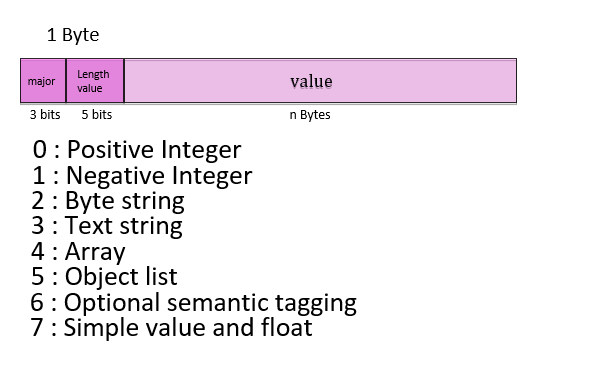
\includegraphics[width=1\columnwidth]{Pictures/cbor1.png}}
\lgf{\caption{Définition des majeurs en CBOR}}
\lge{\caption{Definition of major in CBOR}}
\label{fig-cbor-majeur}
\end{figure}


\lgf{Les cinq bits suivants contiennent soit une valeur soit une longueur indiquant combien d'octets sont nécessaires pour coder la valeur. \ac{CBOR} offre ainsi des optimisations qui permettent de réduire la longueur totale de la structure des données comme nous le verrons par la suite en étudiant les différents types majeurs.}
\lge{The next five bits contain either a value or a length indicating how many bytes are needed to encode the value. \Thus, this type offers optimizations that allow to reduce the total length of the data structure as we will see later when studying the different major types.}

\lgf{\subsection{CBOR en python}}
\lge{\subsection{CBOR in Python}}

\lgf{Les exemples qui vont suivre peuvent être testés sur votre ordinateur avec Python3. Si une erreur se produit au moment de la définition du module \texttt{\Index{cbor2}}, vous devez l'installer sur votre ordinateur en tapant la commande :}
\lge{The following examples can be tested on your computer with Python3. If an error occurs when defining the module \texttt{Index{cbor2}}, you must install it on your computer by typing the command :}

\begin{termc}[backgroundcolor=\color{gray!10}, language=json, basicstyle=\ttfamily\small, escapechar=@]
# @\texttt{pip3 install cbor2}@
\end{termc}


\lgf{\subsection{Type Entier Positif}}
\lgf{\subsection{Type Positive Integer}}


\lgf{\ac{JSON} ne fait pas de différence entre les nombres, entiers, décimaux, positifs ou négatifs. \ac{CBOR} réintroduit une distinction pour optimiser la représentation.}
\lge{\ac{JSON} does not make a difference between numbers, integers, decimals, positive or negative. \ac{CBOR} reintroduces a distinction to optimize the representation.}


      \vspace{1em}

\lgf{Le premier type majeur correspond aux entiers positifs. Il est codé par 3 bits à 0 ; les 5 bits suivants finissent l'octet et, suivant leur valeur, vont avoir une signification différente :}
\lge{The first major type corresponds to the positive integers. It is coded by 3 bits at 0; the 5 following bits end the byte and, according to their value, will have a different meaning:}

\begin{itemize}
    \item 
        \lgf{de 0 à 23, il s'agit de la valeur de l'entier à coder ;}
        \lge{from 0 to 23, it is the value of the integer to be coded;}
    \item 
        \lgf{24 indique que l'entier est codé sur 1 octet qui sera codé dans l'octet suivant ;}
        \lge{24 indicates that the integer is coded on 1 byte which will be coded in the following byte ;}
    \item 
        \lgf{25 indique que l'entier est codé sur 2 octets qui seront codés dans les deux octets suivants ;}
        \lge{25 indicates that the integer is coded on 2 bytes which will be coded in the two following bytes ;}
    \item 
        \lgf{26 indique que l'entier est codé sur 4 octets qui seront codés dans les quatre octets suivants ;}
        \lge{26 indicates that the integer is coded on 4 bytes which will be coded in the four following bytes ;}
    \item 
        \lgf{27 indique que l'entier est codé sur 8 octets qui seront codés dans les huit octets suivants.}
        \lge{27 indicates that the integer is coded on 8 bytes which will be coded in the eight following bytes.}
\end{itemize}

      \vspace{1em}

\lgf{On peut noter qu'il n'y a pas de surcoût pour coder un entier de 0 à 23. Ainsi, la valeur 15 sera codée 0x0F (\texttt{000-0 1111}) tandis que, pour toutes les autres valeurs supérieures, le surcoût ne sera que d'un octet. La valeur 100 sera codé \texttt{000-1 1000}\footnote{\texttt{11000} correspond à 24} suivi du codage sut 1 octet de la valeur 100 (\texttt{0110 0100}).}
\lge{One can note that there is no extra cost to code an integer from 0 to 23. Thus, the value 15 will be coded 0x0F (\texttt{000-0 1111}) while, for all the other higher values, the overcost will be only of one byte. The value 100 will be coded \texttt{000-1 1000}\footnote{\texttt{11000} corresponds to 24} followed by the coding on 1 byte of the value 100 (\texttt{0110 0100}).}



      \vspace{1em}

\pythonlst{cbor-integer-ex1.py}

\lgf{Le programme \pprog{cbor-integer-ex1.py}{cbor-example}  affiche les puissances de $10$ entre $10^0$ et $10^{18}$~:}
\lge{The program \pprog{cbor-integer-ex1.py}{cbor-example} displays the powers of $10$ between $10^0$ and $10^{18}$~:}

\begin{itemize}
    \item 
        \lgf{Ligne 1, le programme importe le module \texttt{\Index{cbor2}} et le renomme pour plus de simplicité \texttt{cbor}.}
        \lge{Line 1, the program imports the module \texttt{Index{cbor2}} and renames it for simplicity \texttt{cbor}.}
    \ligne  
        \lgf{Ligne 5, la boucle permet d'avoir les multiples de 10 (variable \texttt{v)}. }
        \lge{Line 5, the loop allows to have the multiples of 10 (variable \texttt{v)}. }
    \item  
        \lgf{Ligne 6, le module \texttt{cbor} utilise comme pour JSON la méthode \pfunction{cbor2}{dumps} pour sérialiser une structure interne de Python dans la représentation demandée. À l'inverse, la méthode \pfunction{cbor2}{loads} sera utilisée pour importer une structure CBOR dans une représentation interne.}
        \lge{Line 6, the module \texttt{cbor} uses as for JSON the method \pfunction{cbor2}{dumps} to serialize an internal Python structure into the requested representation. Conversely, the \pfunction{cbor2}{loads} method will be used to import a CBOR structure into an internal representation.}
    \item  
        \lgf{Ligne 7, le \texttt{print} permet d'aligner les données pour que l'affichage soit plus clair ; entre les accolades, le premier chiffre indique la position dans les arguments de format ; le second, après le \texttt{:}, le nombre de caractères. Par exemple, \texttt{\{1:30\}} indique l'argument \texttt{v} de format affiché sur 30 caractères.}
        \lge{On line 7, the \texttt{print} is used to align the data so that the display is clearer; between the braces, the first number indicates the position in the format arguments; the second, after the \texttt{:}, the number of characters. For example, \texttt{\{:1:30\}} indicates the format argument \texttt{v} displayed in 30 characters.}
\end{itemize}
 
       \vspace{1em}

\lgf{Le programme donne le résultat suivant~:}
\lge{The program gives the following result:}

\begin{termc}[backgroundcolor=\color{palerod}, language=json, basicstyle=\ttfamily\small, escapechar=@]
 # @\textbf{python3 cbor-integer-ex1.py}@
  0                              1 01
  1                             10 0a
  2                            100 1864
  3                           1000 1903e8
  4                          10000 192710
  5                         100000 1a000186a0
  6                        1000000 1a000f4240
  7                       10000000 1a00989680
  8                      100000000 1a05f5e100
  9                     1000000000 1a3b9aca00
 10                    10000000000 1b00000002540be400
 11                   100000000000 1b000000174876e800
 12                  1000000000000 1b000000e8d4a51000
 13                 10000000000000 1b000009184e72a000
 14                100000000000000 1b00005af3107a4000
 15               1000000000000000 1b00038d7ea4c68000
 16              10000000000000000 1b002386f26fc10000
 17             100000000000000000 1b016345785d8a0000
 18            1000000000000000000 1b0de0b6b3a7640000
\end{termc}

       \vspace{1em}


\lgf{On voit facilement que les valeurs 1 et 10 sont codées sur 1 octet ; que 100 est codé sur 2 octets tandis que les valeurs 1 000 et 10 000 sont codées sur 3 octets. Les valeurs entre 100 000 et 1 000 000 000 nécessitent 5 octets et les valeurs suivantes, 9 octets.}
\lge{It is easy to see that the values 1 and 10 are coded on 1 byte; that 100 is coded on 2 bytes while the values 1 000 and 10 000 are coded on 3 bytes. The values between 100 000 and 1 000 000 000 require 5 bytes and the following values, 9 bytes.}


       \vspace{1em}


\lgf{La taille de la représentation s'adapte à la valeur. Ainsi, il n'est pas nécessaire de définir une taille fixe pour coder une donnée.}
\lge{The size of the representation adapts to the value. Thus, it is not necessary to define a fixed size to encode a data.}

\lgf{On peut aussi noter que comme le type majeur est sur 3 bits, ce type peut être reconnu dans une lecture hexadécimale du résultat car la séquence commence toujours par le symbole \texttt{0} ou \textttt{1}.}
\lge{We can also note that as the major type is on 3 bits, this type can be recognized in a hexadecimal reading of the result because the sequence always starts with the symbol \texttt{0} or \textttt{1}.}

\lgf{\subsection{Type Entier Négatif}}
\lge{\subsection{Type Negative Integer}}


\lgf{Le type majeur entier négatif est à peu près similaire à l'entier positif. Le type majeur est \texttt{001} et le codage de la valeur se fait sur la valeur absolue du nombre à laquelle on retranche 1. Cela évite deux codes différents pour les valeurs 0 et -0.}
\lge{The major type negative integer is roughly similar to the positive integer. The major type is \texttt{001} and the encoding of the value is done on the absolute value of the number to which we subtract 1. This avoids two different codes for the values 0 and -0.}

       \vspace{1em}

\lgf{Ainsi, pour coder -15, on va coder la valeur 14, ce qui donne en binaire 001-1 1110. Ainsi, -24 peut également être codé sur 1 octet tandis que +24 sera codé sur 2 octets.}
\lge{Thus, to code -15, we will code the value 14, which gives in binary 001-1 1110. Thus, -24 can also be coded on 1 byte while +24 will be coded on 2 bytes.}

\pythonlst{cbor-integer-ex2.py}

\lgf{Le programme \pprog{cbor-integer-ex2.py}{cbor-example} reprend le même code que le programme précédent, mais la variable \texttt{v} est initialisée avec la valeur -1. Ce programme va traiter les puissances de 10 négatives.}
\lge{The program \pprog{cbor-integer-ex2.py}{cbor-example} uses the same code as the previous program, but the variable \texttt{v} is initialized with the value -1. This program will process negative powers of 10.}


\begin{termc}[backgroundcolor=\color{palerod}, language=json, basicstyle=\ttfamily\small, escapechar=@]
  # @\textbf{python3.5 cbor-integer-ex2.py}@
  0                             -1 20
  1                            -10 29
  2                           -100 3863
  3                          -1000 3903e7
  4                         -10000 39270f
  5                        -100000 3a0001869f
  6                       -1000000 3a000f423f
  7                      -10000000 3a0098967f
  8                     -100000000 3a05f5e0ff
  9                    -1000000000 3a3b9ac9ff
 10                   -10000000000 3b00000002540be3ff
 11                  -100000000000 3b000000174876e7ff
 12                 -1000000000000 3b000000e8d4a50fff
 13                -10000000000000 3b000009184e729fff
 14               -100000000000000 3b00005af3107a3fff
 15              -1000000000000000 3b00038d7ea4c67fff
 16             -10000000000000000 3b002386f26fc0ffff
 17            -100000000000000000 3b016345785d89ffff
 18           -1000000000000000000 3b0de0b6b3a763ffff
\end{termc}


\lgf{\subsection{Type Séquence binaire ou Chaîne de caractères}}
\lge{\subsection{Type Binary sequence or Character string}}

\lgf{Les séquences binaires et les chaînes de caractères ont le même comportement. Le type majeur est respectivement \texttt{010} et \texttt{011}. Il est suivi par la longueur de la séquence ou de la chaîne. Le même type de codage que pour les entiers est utilisé :}
\lge{Binary sequences and strings have the same behavior. The major type is respectively \texttt{010} and \texttt{011}. It is followed by the length of the sequence or the string. The same type of encoding as for integers is used:}

\begin{itemize}
    \item 
        \lgf{si la longueur est inférieure à 23, elle est codée dans la suite du premier octet. On trouve ensuite le nombre d'octets ou de caractères correspondant à cette longueur ;}
        \lge{if the length is lower than 23, it is coded in the continuation of the first byte. One finds then the number of bytes or characters corresponding to this length;}
    \item  
        \lgf{si la longueur peut être codée dans 1 octet (donc inférieure à 255), la suite du premier octet contient 24 puis l'octet suivant contient la longueur suivie du nombre d'octets ou de caractères correspondant.}
        \lge{if the length can be coded in 1 byte (thus lower than 255), the continuation of the first byte contains 24 then the following byte contains the length followed by the number of bytes or characters corresponding.}
    \item  
        \lgf{si la longueur peut être codée dans 2 octets (donc inférieure à 65535), la suite du premier octet contient 25 puis l'octet suivant contient la longueur suivie du nombre d'octets ou de caractères correspondant.}
        \lge{if the length can be coded in 2 bytes (thus lower than 65535), the continuation of the first byte contains 25 then the following byte contains the length followed by the number of bytes or characters corresponding.}
    \item  
        \lgf{si la longueur peut être codée dans 4 octets, la suite du premier octet contient 26 puis l'octet suivant contient la longueur suivie du nombre d'octets ou de caractères correspondant.}
        \lge{if the length can be coded in 4 bytes, the continuation of the first byte contains 26 then the following byte contains the length followed by the number of bytes or characters corresponding.}
    \item  
        \lgf{si la longueur peut être codée dans 8 octets, la suite du premier octet contient 27 puis l'octet suivant contient la longueur suivie du nombre d'octets ou de caractères correspondant.}
        \lge{if the length can be encoded in 8 bytes, the continuation of the first byte contains 27 then the following byte contains the length followed by the number of bytes or characters corresponding.}
\end{itemize}

       \vspace{1em}

\lgf{Ce codage est aussi assez optimal. Il est rare d'envoyer plus de 23 caractères.}
\lge{This coding is also quite optimal. It is rare to send more than 23 characters.}


\pythonlst{cbor-string.py}

\lgf{Le programme \pprog{cbor-string.py}{cbor-example} montre la représentation de chaînes de caractères de longueur croissante ainsi qu'une séquence binaire~:}
\lge{The program \pprog{cbor-string.py}{cbor-example} shows the representation of strings of increasing length and a binary sequence:}

\begin{itemize}
    \item 
        \lgf{ligne 3, la variable \texttt{i} prend des valeurs de 1 à 9.}
        \lge{line 3, the variable \texttt{i} takes values from 1 to 9.}
    \item  
        \lgf{ligne 6, La multiplication d'une chaîne de caractères par un entier (ligne 4) indique le nombre de répétitions de celle-ci.}
        \lge{line 6, The multiplication of a string by an integer (line 4) indicates the number of repetitions of it.}
    \item  
        \lgf{lignes 8 et 9 montrent le codage d'une chaîne d'octets. La variable bs contient la représentation en CBOR d'une chaîne d'octets Python (représenté par le caractère \texttt{b} avant les guillemets, les valeurs qui ne correspondent pas à des caractères ASCII sont précédées des symboles \texttt{$\backslash$x}). La représentation en hexadécimal de l'objet CBOR est ensuite affichée.}
        \lge{lines 8 and 9 show the encoding of a byte string. The variable bs contains the CBOR representation of a Python byte string (represented by the character \texttt{b} before the quotation marks, the values which do not correspond to ASCII characters are preceded by the symbols \texttt{$\backslash$x}). The hexadecimal representation of the CBOR object is then displayed.}
\end{itemize}

       \vspace{1em}

 
\lgf{Le résultat est le suivant~:}
\lge{The result is as follows:}

\begin{termc}[backgroundcolor=\color{palerod}, language=json, basicstyle=\ttfamily\tiny, escapechar=@]
# @\textbf{python3.5 cbor-string.py}@
  1 674c6f526157414e
  2 6e4c6f526157414e4c6f526157414e
  3 754c6f526157414e4c6f526157414e4c6f526157414e
  4 781c4c6f526157414e4c6f526157414e4c6f526157414e4c6f526157414e
  5 78234c6f526157414e4c6f526157414e4c6f526157414e4c6f526157414e4c6f526157414e
  6 782a4c6f526157414e4c6f526157414e4c6f526157414e4c6f526157414e4c6f526157414e4c6f526157414e
  7 78314c6f526157414e4c6f526157414e4c6f526157414e4c6f526157414e4c6f526157414e4c6f526157414e4c6f526157414e
  8 78384c6f526157414e4c6f526157414e4c6f526157414e4c6f526157414e4c6f526157414e4c6f526157414e4c6f526157414e4c6f526157414e
  9 783f4c6f526157414e4c6f526157414e4c6f526157414e4c6f526157414e4c6f526157414e4c6f526157414e4c6f526157414e4c6f526157...
43010203
\end{termc}


\lgf{Jusqu'à 3 répétitions de la chaîne de caractères "LoRaWAN", le codage de la longueur est optimal (codé sur 2 octets).}
\lge{Up to 3 repetitions of the string "LoRaWAN", the length coding is optimal (coded on 2 bytes).}

\lgf{\subsection{Type tableau}}
\lge{\subsection{Type Array}}

\lgf{Le type tableau va regrouper un ensemble d'éléments. Chacun de ces éléments étant une structure CBOR, la seule information nécessaire pour connaître le début et la fin d'un tableau est son nombre d'éléments. Le type majeur est \texttt{100}. Il existe deux méthodes pour coder la longueur d'un tableau~:}
\lge{The array type will group a set of elements. Each of these elements being a CBOR structure, the only information needed to know the beginning and the end of an array is its number of elements. The major type is \texttt{100}. There are two methods to encode the length of an array:}
\begin{itemize}
    \item 
        \lgf{si celle-ci est connue au moment du codage, il suffit de l'indiquer avec un codage identique à celui utilisé pour indiquer la longueur d'une chaîne de caractères ;}
        \lge{if this one is known at the time of coding, it is enough to indicate it with a coding identical to the one used to indicate the length of a character string ;}
    \item 
        \lgf{si celle-ci n'est pas connue au moment du codage, il existe un code spécial pour indiquer la fin du tableau. Nous en reparlerons par la suite.}
        \lge{if this is not known at the time of coding, there is a special code to indicate the end of the table. We will talk about this later.}
        
\end{itemize}

\pythonlst{cbor-array.py}

\lgf{Le programme \pprog{cbor-array.py}{cbor-example} donne quelques exemples de codage de tableau :}
\lge{The program \pprog{cbor-array.py}{cbor-example} gives some examples of array coding:}

\begin{itemize}
    \item 
        \lgf{\texttt{[1,2,3,4]} défini ligne 3, devient \texttt{8401020304}. On peut deviner la structure du message CBOR : \texttt{0x84} indique un tableau de 4 éléments (attention le décodage n'est pas toujours aussi simple). Les 4 éléments sont des entiers inférieurs à 23 ;}
        \lge{\texttt{[1,2,3,4]} defined on line 3, becomes \texttt{8401020304}. We can guess the structure of the CBOR message: \texttt{0x84} indicates an array of 4 elements (be careful, decoding is not always so simple). The 4 elements are integers lower than 23;}
    \item 
        \lgf{\texttt{[1,[2, 3], 4]} défini ligne 7 devient \texttt{8301\ul{820203}04}. Il s'agit d'un tableau de 3 éléments dont le deuxième est un tableau de deux éléments ;}
        \lge{\texttt{[1,[2, 3], 4]} defined on line 7 becomes \texttt{8301\ul{820203}04}. This is an array of 3 elements, the second of which is an array of two elements;}
    \item 
        \lgf{\texttt{[1000, +20, -10, +100, -30, -50, 12]} défini ligne 11, devient \texttt{871903e814291864 381d38310c}. On peut noter que le codage des éléments est de longueur variable, mais comme chaque élément code sa longueur, il est juste nécessaire d'en connaître le nombre.}
        \lge{\texttt{[1000, +20, -10, +100, -30, -50, 12]} defined on line 11, becomes \texttt{871903e814291864 381d38310c}. Note that the coding of the elements is of variable length, but as each element codes its length, it is only necessary to know the number of elements.}
\end{itemize}

\lgf{\subsection{Type Map (Liste de paires)}}
\lgf{\subsection{Type Map (List of pairs)}}



\lgf{Le type Liste de paires ou Map est indiqué par la valeur \texttt{101}. Il fonctionne de la même manière que les tableaux en comptant le nombre d'éléments. Mais cette fois-ci, la valeur représente une paire, c'est-à-dire deux objets CBOR consécutifs.}
\lge{The type List of pairs or Map is indicated by the value \texttt{101}. It works in the same way as arrays by counting the number of elements. But this time, the value represents a pair, i.e. two consecutive CBOR objects.}


\pythonlst{cbor-mapped.py}

\lgf{Le programme \pprog{cbor-mapped.py}{cbor-example} donne un exemple d'encodage. A noter que la structure à encoder n'est pas directement compatible avec JSON\footnote{json.\pfunction{json}{dumps} aurait converti les clés numériques en chaînes de caractères \texttt{'\{"type": "hamster", "2": "program", "taille": 300, "15": 113\}'}}, certaines clés ne sont pas des chaînes de caractères.}
\lge{The program \pprog{cbor-mapped.py}{cbor-example} gives an example of encoding. Note that the structure to be encoded is not directly compatible with JSONfootnote{json.\pfunction{json}{dumps} would have converted the numeric keys into strings \texttt{'\{"type": "hamster", "2": "program", "taille": 300, "15": 113\}'}}, some keys are not strings.}


       \vspace{1em}


\lgf{Le résultat est \texttt{a464747970656768616d73746572667461696c6c6519012c026770726f6772 616d0f1871} ce qui n'est pas très facile à lire. }
\lge{The result is \texttt{a464747970656768616d73746572667461696c6c6519012c026770726f6772 616d0f1871} which is not very easy to read. }



\subsubsection{cbor.me}

\begin{wrapfigure}{r}{3cm}
\Youtube{https://youtu.be/h1XnaFy_FoI}
\end{wrapfigure}

\lgf{Le site web \url{https://cbor.me} permet de faire automatiquement le codage dans un sens ou dans l'autre.
La colonne de gauche représente la donnée en JSON et celle de droite en CBOR (dite "représentation canonique" qui facilite la lecture). En ayant entré la séquence hexadécimale ci-dessus, le site la présente comme indiqué figure~\vref{fig-cbor-me}.
La partie CBOR est indexée et commentée pour rendre l'objet CBOR plus lisible. Il peut également être traduit dans un équivalent JSON, bien que certaines clés restent numériques.}
\lge{The web site \url{https://cbor.me} allows to do automatically the encoding in a direction or in the other.
The left column represents the data in JSON and the right one in CBOR (called "canonical representation" which facilitates the reading). Having entered the above hexadecimal sequence, the site presents it as shown in figure~\vref{fig-cbor-me}.
The CBOR part is indexed and commented to make the CBOR object more readable. It can also be translated into a JSON equivalent, although some keys remain numeric.}


\begin{figure}[tbp]
\centerline{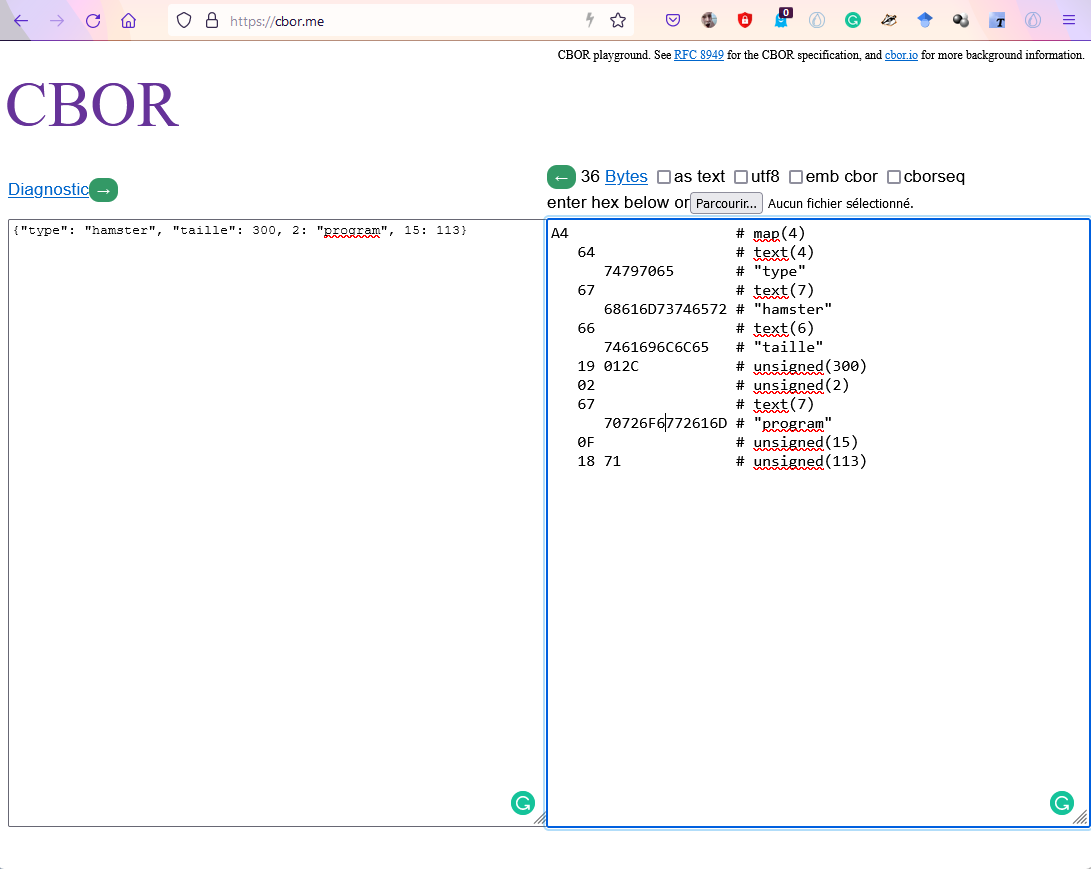
\includegraphics[width=1\columnwidth]{Pictures/cbor-me.png}}
\lgf{\caption{Définition des majeurs en CBOR}}
\lge{\caption{Definition of major in CBOR}}
\label{fig-cbor-me}
\end{figure}

\lgf{Sur ces exemples, on peut voir que CBOR est beaucoup plus permissif et complet que JSON, le premier champ des map CBOR peut être numérique et n'a pas à être unique dans toute la structure. Néanmoins  CBOR
définit un mode strict dans lequel ces clés doivent être codées en ASCII et unique pour être compatibles avec
JSON. Si une clé est répété plusieurs fois dans une structure CBOR, il traiter directement l'information dans la structure CBOR et ne pas chercher à la convertir ou la désérialiser car il y a un risque de perte d'information. }
\lge{On these examples, we can see that CBOR is much more permissive and complete than JSON, the first field of the CBOR map can be numeric and does not have to be unique in the whole structure. Nevertheless CBOR
defines a strict mode in which these keys must be ASCII encoded and unique to be compatible with
JSON. If a key is repeated several times in a CBOR structure, it is necessary to process the information directly in the CBOR structure and not to try to convert or deserialize it because there is a risk of losing information. }


\lgf{\subsection{Type étiquette}}
\lge{\subsection{Type Tag}}


\lgf{CBOR enrichit le typage des données ; ce qui permet de manipuler plus facilement des données. Par exemple, une chaîne de caractères peut représenter une date, une URI, voire une URI codée en base 64. Le type \texttt{110} peut être suivi d'une valeur ou \Index{tag} dont une liste exhaustive est maintenue parl'IANA\footnote{\url{https://www.iana.org/assignments/cbor-tags/cbor-tags.xhtml}}.}
\lge{CBOR enriches the typing of data; this makes it easier to manipulate data. For example, a character string can represent a date, a URI, or even a URI encoded in base 64. The type \texttt{110} can be followed by a value or \Index{tag} of which an exhaustive list is maintained by the IANAfootnote{url{https://www.iana.org/assignments/cbor-tags/cbor-tags.xhtml}}.}

\pythonlst{cbor-tag.py}

\lgf{Par exemple, le programme \pprog{cbor-tag.py}{cbor-example} retourne les résultats suivants~:}
\lge{For example, the program \pprog{cbor-tag.py}{cbor-example} returns the following results:}


\begin{termc}[backgroundcolor=\color{palerod}, language=json, basicstyle=\ttfamily\small, escapechar=@]
# @\textbf{python3.5 cbor-tag.py}@
2018-05-22
c074323031382d30352d32325430303a30303a30305a
2018-05-22 00:00:00+00:00
43010203
<class 'datetime.datetime'>
\end{termc}


\lgf{La représentation canonique montre plus facilement le tag dans la séquence binaire :}
\lge{The canonical representation shows more easily the tag in the binary sequence:}


\begin{termc}[backgroundcolor=\color{palerod}, language=json, basicstyle=\ttfamily\small, escapechar=@]
C0                                      # tag(0)
   74                                   # text(20)
      323031382D30352D32325430303A30303A30305A # "2018-05-22T00:00:00Z"
\end{termc}

\lgf{Le tag 0 implique un format normalisé pour la date ; d'où l'ajout des heures, minutes et secondes, alors qu'elles n'ont pas été spécifiées initialement. On peut également remarquer que \pfunction{cbor2}{loads} retourne un type \texttt{date} et non une chaîne de caractères.}
\lge{The tag 0 implies a normalized format for the date; hence the addition of hours, minutes and seconds, even though they were not initially specified. We can also notice that \pfunction{cbor2}{loads} returns a type \texttt{date} and not a character string.}


\lgf{\subsection{Le type flottant et valeurs particulières}}
\lge{\subsection{The floating type and particular values}}


\lgf{Le dernier type majeur (111) permet de coder les nombres flottants en utilisant la représentation définie par l'\Index{IEEE 754}. Suivant la taille de la représentation, la suite de l'octet contient les valeurs 25 (demi précision sur 16 bits), 26 (simple précision sur 32 bits) ou 27 (double précision sur 64 bits).}
\lge{The last major type (111) allows to encode floating numbers by using the representation defined by the \Index{IEEE 754}. According to the size of the representation, the continuation of the byte contains the values 25 (half precision on 16 bits), 26 (simple precision on 32 bits) or 27 (double precision on 64 bits).}


\lgf{Ce type permet également de coder les valeurs définies par JSON : True (valeur 20), False (valeur 21) ou None (valeur 22).}
\lge{This type also allows to encode the values defined by JSON: True (value 20), False (value 21) or None (value 22).}


\lgf{Finalement, ce type peut indiquer la fin d'un tableau ou d'une liste de paires quand la taille n'est pas connue au début du codage.}
\lge{Finally, this type can indicate the end of an array or a list of pairs when the size is not known at the beginning of the coding.}


\lgf{\section{Questions sur CBOR}}
\lge{\section{Questions about CBOR}}

\Question{\lgf{Avantages de CBOR}\lge{Benefits of CBOR}}
{
\lgf{Quel sont les avantage de CBOR par rapport à JSON (2 réponses) ?}
\lge{What are the advantages of CBOR over JSON (2 answers)?}

\begin{itemize}[label=$\square$]
   \item \Correct{
     \lgf{Il est plus compact dans la représentation des données.}
     \lge{It is more compact in its data representation.}
    }
   \item \Wrong{
    \lgf{Il permet de représenter des nombres flottants.}
    \lge{It allows to represent floating numbers.}
    }
   \item \Wrong{
    \lgf{Il compresse les chaînes de caractères. }
    \lge{It compresses strings. }
    }
   \item \Correct{
    \lgf{Il est plus simple à implémenter.}
    \lge{It is easier to implement.}
    }
 \end{itemize}
   
 }
{
\lgf{CBOR ne compresse pas les chaînes de caractères. Il ajoute juste leur longueur. CBOR et JSON codent tous les deux des nombres flottants, ce n'est donc pas un avantage de CBOR. Par contre, le fait d'utiliser des valeurs binaires au lieu de l'ASCII pour représenter les nombres, de ne pas avoir de crochets ou accolades, permet d'avoir une représentation beaucoup plus compacte. Les petites valeurs numériques sont représentées sans surcoût. Réaliser un codeur ou un décodeur de CBOR est beaucoup plus simple qu'en JSON car la représentation des données est beaucoup plus stricte (pas d'espace, pas de retour à la ligne... ). Les deux représentations permettent d'utiliser des nombres flottant donc aucune n'a d'avantage sur ce point.}
\lge{CBOR does not compress strings. It just adds their length. Both CBOR and JSON encode floating-point numbers, so this is not an advantage of CBOR. On the other hand, using binary values instead of ASCII to represent numbers, not having brackets or braces, makes for a much more compact representation. Small numerical values are represented without any additional cost. Creating a CBOR encoder or decoder is much simpler than in JSON because the data representation is much stricter (no spaces, no line breaks, etc.). Both representations allow to use floating numbers so neither has an advantage on this point.}


}

\Question{\lgf{Flottant}\lge{Floating}}{
\lgf{Un flottant est-il toujours plus compact en CBOR qu'en JSON ? - Vous pouvez vous aider de \url{https://cbor.me}}
\lge{Is a float always more compact in CBOR than in JSON? - You can help yourself with \url{https://cbor.me}}


\begin{itemize}[label=$\circ$]
   \item \Wrong{
    \lgf{Oui, c'est le but de CBOR.}
    \lge{Yes, that is the goal of CBOR.}
    }
   \item \Wrong{
    \lgf{Oui, pour les flottants qui ont la partie décimale à 0.}
    \lge{Yes, for floats that have the decimal part at 0.}
    }
   \item \Wrong{
    \lgf{Oui, pour les flottants de petite précision (jusqu'au centième).}
    \lge{Yes, for small precision floats (up to a hundredth).}
    }
   \item \Correct{
    \lgf{Oui, pour les flottants de grande précision (6 chiffres après la virgule).}
    \lge{Yes, for high precision floats (6 digits after the decimal point).}
    }
 \end{itemize}
}{
\lgf{Un nombre flottant, quelle que soit sa valeur, est représenté par 8 octets en CBOR. En JSON, un nombre flottant est représenté par une chaîne de caractères. Donc "3.0" nécessite 3 caractères, donc plus compacte que CBOR. Mais "3.1415926" est codé sur 9 caractères donc moins compacte que CBOR.}
\lge{A floating number, whatever its value, is represented by 8 bytes in CBOR. In JSON, a floating number is represented by a string. So "3.0" needs 3 characters, so it is more compact than CBOR. But "3.1415926" is coded on 9 characters so less compact than CBOR.}

}

\Question{lgf{Chaîne de caractères}\lgf{Strings}}
{
\lgf{Soit une chaîne de caractères en CBOR.}
\lge{Consider a string in CBOR.}

\begin{itemize}[label=$\circ$]
   \item \Wrong{
    \lgf{Elle est compressée avec un algorithme entropique (e.g. codage de Huffman).}
    \lge{It is compressed with an entropy algorithm (e.g. Huffman coding).}
    }
   \item \Correct{
    \lgf{Elle peut contenir des caractères accentués.}
    \lge{It can contain accented characters.}
    }
   \item \Wrong{
    \lgf{Chaque caractère est codé sur 6 bits.}
    \lge{Each character is coded on 6 bits.}
    }
 \end{itemize}

}{
\lgf{A string is a sequence of bytes. It is possible to use representations offering accented characters (even emoticons). However, CBOR does not compress data.}
}

\Question{\lgf{Taille variable}\lge{Variable length}}
{
\lgf{En CBOR, la taille d'un entier varie en fonction de sa valeur !}
\lge{In CBOR, the size of an integer varies according to its value!}

\begin{itemize}[label=$\circ$]
   \item \Correct{\Vrai}
   \item \Wrong{\Faux}
   \item \Wrong{
    \lgf{Ça dépend de la manière dont on a déclaré cet entier.}
    \lge{It depends on how this integer was declared.}
    }
 \end{itemize}

}{
\lgf{Oui, un entier inférieur à 23 sera codé sur un seul octet. Pour les valeurs plus grandes, il faut ajouter la longueur.}
\lge{Yes, an integer less than 23 will be encoded on a single byte. For larger values, the length must be added.}
}

\Question{\lgf{Tableau}\lge{Array}}
{
\lgf{En CBOR, un tableau peut contenir des objets de types différents.}
\lge{In CBOR, an array can contain objects of different types.}

\begin{itemize}[label=$\circ$]
   \item \Correct{\Vrai}
   \item \Wrong{\Faux}
   \item \Wrong{
   \lgf{Ça dépend de la manière dont on a déclaré ce tableau.}
   \lge{It depends on how this table was declared.}
   }
 \end{itemize}
}
{
\lgf{Vrai, on a la même flexibilité qu'en JSON en imbriquant n'importe quel type de données dans un tableau.}
\lge{True, we have the same flexibility as in JSON by nesting any data type in an array.}
}


\Question{\lgf{Fraction}\lge{Fractional}}
{
\lgf{On veut définir un tableau de deux éléments comme une fraction. Quel tag devra précéder la structure ?
(vous pouvez vous aider du \rfc{8949}).}
\lge{We want to define an array of two elements as a fraction. What tag should precede the structure?
(you can use the \rfc{8949}).}
}
{
\lgf{Il s'agit du tag 4, voir le chapitre \textbf{3.4.4. Decimal Fractions and Bigfloats} du \rfc{8949}.}
\lge{This is tag 4, see the chapter \textbf{3.4.4. Decimal Fractions and Bigfloats} of the \rfc{8949}.}
}

\section{SenML}

\lgf{\ac{SenML} est une une spécification qui exploite JSON ou CBOR. Elle liste un ensemble de noms/unités/mesures et les standardise en un nom de clé unique. En utilisant cette standardisation, on facilite l'interopérabilité. Les clés et valeurs sont donc règlementées et typées pour éviter tous conflits d'interopérabilité. Le format est défini dans la \rfc{8428} et repose sur une structure de tableau regroupant des objets comme le montre la figure suivante tirée de la RFC.}
\lge{\SenML is a specification that leverages JSON or CBOR. It lists a set of names/units/measures and standardizes them into a unique key name. By using this standardization, interoperability is facilitated. The keys and values are therefore regulated and typed to avoid any interoperability conflicts. The format is defined in the RFC{8428} and is based on a table structure grouping objects as shown in the following figure taken from the RFC.}


\begin{termc}[backgroundcolor=\color{palerod}, language=json, basicstyle=\ttfamily\small, escapechar=@]
[
 {"bn" : "urn:dev:ow:10e2073a01080063", "bt":1.320067464e+09,
  "bu" : "\%RH", "v":21.2},
 {"t":10, "v":21.3},
 {"t":20, "v":21.4},
 {"t":30, "v":21.4},
...
\end{termc}

\lgf{SenML définit les clés utilisées dans l’objet. Pour avoir une notation compacte, elles sont limitées à 1 ou 2 caractères. Parmi elles, ”bn” indique un nom de base et ”n” le nom d’un appareil. Si plusieurs appareils envoient la partie commune de l’identifiant de l’appareil, on peut mettre le ”bn” pour éviter de le répéter à chaque fois.}
\lge{SenML defines the keys used in the object. To have a compact notation, they are limited to 1 or 2 characters. Among them, "bn" indicates a base name and "n" the name of a device. If several devices send the common part of the device identifier, we can put the "bn" to avoid repeating it each time.}

\lgf{Le temps de base (ou ”bt”) est également un moyen de compacter la notation du temps. Le temps (”t”) donne le décalage et conduit à une valeur plus petite comme on le voit dans l’exemple.}
\lge{The base time (or "bt") is also a way to compact the time notation. The time ("t") gives the offset and leads to a smaller value as seen in the example.}


\lgf{L’unité de base (”bu”) indique l’unité par défaut si les autres objets ne portent pas de mot clé indiquant l’unité (”u”).}
\lge{The base unit ("bu") indicates the default unit if the other objects do not have a keyword indicating the unit ("u").}

\lgf{La \rfc{8428} définit une liste d’unités telles que le kilogramme (”kg”), le volt (”V”), etc. Dans l’exemple, ”\%RH” désigne un pourcentage d’humidité relative. Une valeur numérique utilise la lettre ”v”, une chaîne de caractères utilise la touche ”vs”.}
\lge{The \rfc{8428} defines a list of units such as kilogram ("kg"), volt ("V"), etc. In the example, "\%RH" refers to a percentage of relative humidity. A numeric value uses the letter "v", a string uses the "vs" key.}


\lgf{CBOR utilise la même structure mais les petits nombres entiers positifs et négatifs sont substitués dans les clés des objets de CBOR : ”bn”, ”bt”, ”bu” seront respectivement représentés par -1, -2 et -3 et ”n”, ”t”, ”u” par +0, +2 et +6.}
\lge{CBOR uses the same structure but small positive and negative integers are substituted in the keys of CBOR objects: "bn", "bt", "bu" will be represented by -1, -2 and -3 respectively and "n", "t", "u" by +0, +2 and +6.}


